\documentclass[12pt]{article}
\usepackage{amsmath,amssymb}
\usepackage{booktabs}
\usepackage{multirow}
\usepackage{geometry}
\usepackage{array}
\usepackage{caption}
\usepackage{graphicx}
\usepackage{hyperref}
\geometry{margin=1in}

\title{Simulation Study: Three-Time-Point SNTTEM\\[0.3em]
\large Data-Generating Mechanism and Results by Scenario}
\date{}

\begin{document}
\maketitle
\tableofcontents
\newpage

%%==========================================================================
\section{Data-Generating Mechanism}
%%==========================================================================

\subsection{Common Temporal Structure}

We simulate longitudinal data for $n$ individuals over three time points
$t\in\{0,1,2\}$.  At each time point we observe a time-varying covariate
$L_t$, an eligibility indicator $I_t\in\{0,1\}$, and a binary treatment
$A_t\in\{0,1\}$.  The temporal ordering is
\[
  I_0,\,L_0,\,A_0
  \;\longrightarrow\;
  I_1,\,L_1,\,A_1
  \;\longrightarrow\;
  I_2,\,L_2,\,A_2
  \;\longrightarrow\;
  Y.
\]
The DGP is governed by five scalar parameters:
\begin{itemize}
  \item $\psi_{03},\psi_{13},\psi_{23}$: structural blip parameters encoding
        the causal effect of treatment at each time point;
  \item $p_I\in(0,1)$: marginal probability of eligibility at times 1 and 2;
  \item $p_h\in(0,1)$: probability that treatment is \emph{held}
        (i.e.\ unchanged) from one period to the next.
\end{itemize}

\subsection{Time $t=0$}

Every individual is eligible at baseline ($I_0=1$).
\[
  L_0 \;\sim\; \mathrm{Uniform}(0,\,0.5),
  \qquad
  A_0\mid L_0 \;\sim\; \mathrm{Bernoulli}\!\left(\mathrm{expit}(-1+L_0)\right),
\]
where $\mathrm{expit}(x)=e^x/(1+e^x)$.

\subsection{Times $t=1$ and $t=2$}

The covariate $L_t$ is a truncated version of a latent normal draw.
We use the clipping operator $\mathrm{clip}:\mathbb{R}\to[a,b]$, defined for
bounds $a < b$ as
\begin{equation}
  \mathrm{clip}(x;\,a,\,b)
  \;=\; \max\!\bigl(a,\;\min(b,\,x)\bigr)
  \;=\;
  \begin{cases}
    a & \text{if } x < a,\\
    x & \text{if } a \le x \le b,\\
    b & \text{if } x > b.
  \end{cases}
  \label{eq:clip}
\end{equation}
This operation hard-limits the support of $L_t$ to the interval $[a,b]$,
replacing any draw below $a$ with $a$ and any draw above $b$ with $b$, while
leaving values already within $[a,b]$ unchanged.

For each $t\in\{1,2\}$:
\begin{align*}
  I_t &\;\sim\; \mathrm{Bernoulli}(p_I),\\
  L_t^* \mid A_{t-1} &\;\sim\; \mathcal{N}(-0.5\,A_{t-1},\;1),\\
  L_t &\;=\; \mathrm{clip}(L_t^*;\,-1.5,\,-0.5),\\
  A_t \mid A_{t-1} &\;=\;
  \begin{cases}
    A_{t-1}   & \text{with probability }p_h,\\
    1-A_{t-1} & \text{with probability }1-p_h.
  \end{cases}
\end{align*}
The clipping bounds $[-1.5,\,-0.5]$ ensure that $L_t$ has bounded, strictly
negative support regardless of $A_{t-1}$.  Concretely: without treatment
($A_{t-1}=0$) the latent draw is $L_t^*\sim\mathcal{N}(0,1)$, and with
treatment ($A_{t-1}=1$) it is $L_t^*\sim\mathcal{N}(-0.5,1)$; in both cases
the clip truncates the distribution to $[-1.5,\,-0.5]$, keeping the covariate
in a regime where the blip functions $\gamma_{13}$ and $\gamma_{23}$ (which
depend on $1+L_t \in [0.5,\,1.5]$) remain positive and bounded away from zero.

\subsection{Structural Blip Functions}

The structural blip functions represent the causal effect on the outcome
of incrementing treatment by one unit at time $t$, conditional on the
covariate history:
\begin{align}
  \gamma_{03}(L_0;\,\psi_{03}) &= \psi_{03}\,L_0,\label{eq:blip0}\\
  \gamma_{13}(L_1;\,\psi_{13}) &= \psi_{13}\,(1+L_1),\label{eq:blip1}\\
  \gamma_{23}(L_2;\,\psi_{23}) &= \psi_{23}\,(1+L_2).\label{eq:blip2}
\end{align}

\subsection{Binary Outcome DGP}

Used in Scenarios~S1 (null) and S2 (non-null).  The outcome follows a
log-linear model $Y\sim\mathrm{Bernoulli}(\exp(\eta))$, where
\begin{align}
  \eta \;=\; {}&-1.5
  + \psi_{03}\,L_0\,A_0 \notag\\
  &+\; I_1\,\psi_{13}\,(1+L_1)\,(A_1-A_0)
   \;+\; (1-I_1)\,\psi_{13}\,\tfrac{L_1}{3}\,(A_1-A_0) \notag\\
  &+\; I_2\,\psi_{23}\,(1+L_2)\,(A_2-A_1)
   \;+\; (1-I_2)\,\psi_{23}\,\tfrac{L_2}{3}\,(A_2-A_1).\label{eq:eta}
\end{align}
For eligible individuals ($I_t=1$) the blip is $\gamma_t(L_t)$;
for ineligible individuals ($I_t=0$) it is attenuated to
$\gamma_t(L_t)\cdot L_t/[3(1+L_t)]$.

\subsection{Continuous Outcome DGP}

Used in Scenarios~S3--S5 ($\psi=1$, varying noise).
The outcome follows a Gaussian model
$Y\sim\mathcal{N}(\mu_Y,\,\sigma_Y^2)$, where
\begin{align}
  \mu_Y &= -1.5
    + \psi_{03}\,L_0\,A_0
    + \psi_{13}\,(1+L_1)\,(A_1-A_0)
    + \psi_{23}\,(1+L_2)\,(A_2-A_1),\label{eq:mu_cont}\\
  \sigma_Y &= \sigma\,\bigl[A_0+(A_1-A_0)^2+(A_2-A_1)^2\bigr]+1.\label{eq:sigma_cont}
\end{align}
Unlike the binary DGP, the mean outcome \eqref{eq:mu_cont} contains no
eligibility interaction: the blip $\gamma_t(L_t)$ applies equally to
all individuals.  The heteroscedasticity parameter $\sigma\geq0$
scales noise with treatment activity; $\sigma=0$ gives a deterministic outcome.

%%==========================================================================
\section{Nuisance Models}
%%==========================================================================

All estimators rely on the following nuisance functions, estimated
via two-fold cross-fitting in each Monte Carlo iteration:
\begin{itemize}
  \item Propensity scores $\pi_t = P(A_t=1\mid\bar{L}_t,A_{t-1})$,
        $t\in\{0,1,2\}$.
  \item Outcome regressions $\mu_{t3}$ constructed sequentially from the
        SNTTEM backward induction, using doubly-robust (DR) pseudo-outcomes
        at each step.
\end{itemize}
Within each fold, each nuisance function is estimated by an
equal-weight ensemble of:
\begin{enumerate}
  \item Random Forest (200 trees);
  \item Gradient Boosting Machine (200 trees, max depth 4, learning rate 0.1);
  \item Degree-3 polynomial Logistic/Linear Regression.
\end{enumerate}

%%==========================================================================
\section{Estimators}
%%==========================================================================

Three estimators of $\boldsymbol{\psi}=(\psi_{03},\psi_{13},\psi_{23})$
are compared.  All solve a system of three estimating equations via
M-estimation (root-finding with \texttt{scipy.optimize.fsolve}).

\paragraph{Three-step estimator (TS).}
Conventional sequential regression approach.  Uses eligibility-based
SNTTEM blip-down with multiplicative (binary) or linear (continuous)
transformations.

\paragraph{Simple g-estimator (SG).}
Doubly-robust SNTTEM estimator.  Uses eligibility-modified weights
$w_t^I = w_t^{1-I_t}$ in all three estimating equations, exploiting the
eligibility indicator to identify blip parameters only from eligible subjects
while borrowing efficiency from ineligible subjects through the outcome
regression.

\paragraph{GMM estimator.}
Optimal inverse-covariance combination of TS and SG, computed via
200 bootstrap resamples of the nuisance-fitted data per iteration.


%%==========================================================================
\section{Simulation Design}
%%==========================================================================

All scenarios cross $p_h\in\{0.4,\,0.6,\,0.8\}$ with
$p_I\in\{0.25,\,0.50,\,0.75,\,1.00\}$, giving 12 cells per scenario.
Each cell uses 100 Monte Carlo iterations (seed 3411).
Table~\ref{tab:design} summarises the five scenarios.

\begin{table}[htbp]
\centering
\caption{Summary of simulation scenarios.}
\label{tab:design}
\small
\begin{tabular}{cllccl}
\toprule
Scenario & Outcome & True $\boldsymbol{\psi}$ & $\sigma$ & $n$ & Estimating eqs.\\
\midrule
S1 & Binary   & $(0,0,0)$   & ---  & 6000 & Multiplicative blip-down \\
S2 & Binary   & $(1,1,1)$   & ---  & 6000 & Multiplicative blip-down \\
S3 & Continuous & $(1,1,1)$ & 0    & 4000 & Linear blip-down \\
S4 & Continuous & $(1,1,1)$ & 10   & 4000 & Linear blip-down \\
S5 & Continuous & $(1,1,1)$ & 20   & 4000 & Linear blip-down \\
\bottomrule
\end{tabular}
\end{table}

\noindent Under the null ($\boldsymbol{\psi}=\mathbf{0}$) the multiplicative and linear
estimating equations are algebraically equivalent (since
$e^{-\gamma_t\cdot 0}=1$ and $-\gamma_t\cdot 0=0$), so S1 applies
to both binary and continuous estimators simultaneously.

%%==========================================================================
\section{Results}
%%==========================================================================

Tables~\ref{tab:s1_psi03}--\ref{tab:s5_psi23} report empirical
\emph{bias} ($\hat\psi - \psi_{\mathrm{true}}$) and Monte Carlo
\emph{variance} over 100 iterations for each method, scenario, and
parameter.  Results are grouped by $p_h$ within each table.

%%--------------------------------------------------------------------------
\subsection{Scenario S1: Null ($\psi_{03}=\psi_{13}=\psi_{23}=0$, Binary DGP, $n=6000$)}
%%--------------------------------------------------------------------------

\begin{table}[htbp]
\centering
\caption{S1 --- Empirical bias and variance for $\hat\psi_{03}$.
         True value: $\psi_{03}=0$.}
\label{tab:s1_psi03}
\small
\begin{tabular}{cc rr rr rr}
\toprule
& & \multicolumn{2}{c}{Three-step} & \multicolumn{2}{c}{Simple g-est.} & \multicolumn{2}{c}{GMM} \\
\cmidrule(lr){3-4}\cmidrule(lr){5-6}\cmidrule(lr){7-8}
$p_h$ & $p_I$ & Bias & Var & Bias & Var & Bias & Var \\
\midrule
\multirow{4}{*}{0.4}
 & 0.25 & $\phantom{-}0.0149$ & 0.5701 & $\phantom{-}0.0158$ & 0.4560 & $-0.1452$ & 0.4505 \\
 & 0.50 & $\phantom{-}0.0144$ & 0.5681 & $\phantom{-}0.0260$ & 0.3945 & $-0.1046$ & 0.3706 \\
 & 0.75 & $\phantom{-}0.0139$ & 0.5675 & $\phantom{-}0.0135$ & 0.3220 & $-0.0865$ & 0.2962 \\
 & 1.00 & $\phantom{-}0.0145$ & 0.5687 & $\phantom{-}0.0069$ & 0.2397 & $-0.0583$ & 0.2344 \\
\midrule
\multirow{4}{*}{0.6}
 & 0.25 & $\phantom{-}0.0122$ & 0.1811 & $\phantom{-}0.0132$ & 0.1516 & $-0.0486$ & 0.1463 \\
 & 0.50 & $\phantom{-}0.0130$ & 0.1811 & $\phantom{-}0.0143$ & 0.1398 & $-0.0432$ & 0.1362 \\
 & 0.75 & $\phantom{-}0.0127$ & 0.1812 & $\phantom{-}0.0177$ & 0.1387 & $-0.0190$ & 0.1365 \\
 & 1.00 & $\phantom{-}0.0125$ & 0.1812 & $\phantom{-}0.0159$ & 0.1164 & $-0.0191$ & 0.1083 \\
\midrule
\multirow{4}{*}{0.8}
 & 0.25 & $\phantom{-}0.0077$ & 0.0948 & $\phantom{-}0.0070$ & 0.0855 & $-0.0205$ & 0.0841 \\
 & 0.50 & $\phantom{-}0.0080$ & 0.0947 & $\phantom{-}0.0082$ & 0.0826 & $-0.0180$ & 0.0791 \\
 & 0.75 & $\phantom{-}0.0078$ & 0.0946 & $\phantom{-}0.0097$ & 0.0848 & $-0.0151$ & 0.0849 \\
 & 1.00 & $\phantom{-}0.0076$ & 0.0948 & $\phantom{-}0.0063$ & 0.0763 & $-0.0162$ & 0.0740 \\
\bottomrule
\end{tabular}
\end{table}

\begin{table}[htbp]
\centering
\caption{S1 --- Empirical bias and variance for $\hat\psi_{13}$.
         True value: $\psi_{13}=0$.}
\label{tab:s1_psi13}
\small
\begin{tabular}{cc rr rr rr}
\toprule
& & \multicolumn{2}{c}{Three-step} & \multicolumn{2}{c}{Simple g-est.} & \multicolumn{2}{c}{GMM} \\
\cmidrule(lr){3-4}\cmidrule(lr){5-6}\cmidrule(lr){7-8}
$p_h$ & $p_I$ & Bias & Var & Bias & Var & Bias & Var \\
\midrule
\multirow{4}{*}{0.4}
 & 0.25 & $\phantom{-}0.0598$ & 0.4521 & $\phantom{-}0.0512$ & 0.3721 & $-0.0386$ & 0.3879 \\
 & 0.50 & $\phantom{-}0.0042$ & 0.2284 & $-0.0035$ & 0.1712 & $-0.0678$ & 0.1696 \\
 & 0.75 & $\phantom{-}0.0007$ & 0.1437 & $-0.0073$ & 0.1195 & $-0.0550$ & 0.1164 \\
 & 1.00 & $\phantom{-}0.0001$ & 0.1060 & $-0.0107$ & 0.0948 & $-0.0489$ & 0.0924 \\
\midrule
\multirow{4}{*}{0.6}
 & 0.25 & $\phantom{-}0.0246$ & 0.2917 & $\phantom{-}0.0240$ & 0.2775 & $-0.0376$ & 0.2771 \\
 & 0.50 & $\phantom{-}0.0128$ & 0.1460 & $\phantom{-}0.0141$ & 0.1276 & $-0.0286$ & 0.1245 \\
 & 0.75 & $\phantom{-}0.0220$ & 0.0859 & $\phantom{-}0.0183$ & 0.0748 & $-0.0056$ & 0.0735 \\
 & 1.00 & $\phantom{-}0.0127$ & 0.0711 & $\phantom{-}0.0116$ & 0.0645 & $-0.0090$ & 0.0611 \\
\midrule
\multirow{4}{*}{0.8}
 & 0.25 & $\phantom{-}0.0488$ & 0.3419 & $\phantom{-}0.0482$ & 0.3224 & $-0.0085$ & 0.3266 \\
 & 0.50 & $\phantom{-}0.0345$ & 0.1432 & $\phantom{-}0.0359$ & 0.1331 & $\phantom{-}0.0080$ & 0.1282 \\
 & 0.75 & $\phantom{-}0.0096$ & 0.0775 & $\phantom{-}0.0074$ & 0.0708 & $-0.0200$ & 0.0711 \\
 & 1.00 & $\phantom{-}0.0095$ & 0.0677 & $\phantom{-}0.0104$ & 0.0610 & $-0.0084$ & 0.0593 \\
\bottomrule
\end{tabular}
\end{table}

\begin{table}[htbp]
\centering
\caption{S1 --- Empirical bias and variance for $\hat\psi_{23}$.
         True value: $\psi_{23}=0$.
         TS and SG share the same third estimating equation, so their
         $\hat\psi_{23}$ estimates are identical by construction.}
\label{tab:s1_psi23}
\small
\begin{tabular}{cc rr rr rr}
\toprule
& & \multicolumn{2}{c}{Three-step} & \multicolumn{2}{c}{Simple g-est.} & \multicolumn{2}{c}{GMM} \\
\cmidrule(lr){3-4}\cmidrule(lr){5-6}\cmidrule(lr){7-8}
$p_h$ & $p_I$ & Bias & Var & Bias & Var & Bias & Var \\
\midrule
\multirow{4}{*}{0.4}
 & 0.25 & $-0.0203$ & 0.2057 & $-0.0203$ & 0.2057 & $-0.0321$ & 0.1914 \\
 & 0.50 & $-0.0195$ & 0.0927 & $-0.0195$ & 0.0927 & $-0.0354$ & 0.0916 \\
 & 0.75 & $-0.0021$ & 0.0499 & $-0.0021$ & 0.0499 & $-0.0200$ & 0.0502 \\
 & 1.00 & $-0.0061$ & 0.0406 & $-0.0061$ & 0.0406 & $-0.0221$ & 0.0401 \\
\midrule
\multirow{4}{*}{0.6}
 & 0.25 & $-0.0235$ & 0.1998 & $-0.0235$ & 0.1998 & $-0.0247$ & 0.1862 \\
 & 0.50 & $-0.0139$ & 0.0896 & $-0.0139$ & 0.0896 & $-0.0265$ & 0.0881 \\
 & 0.75 & $\phantom{-}0.0037$ & 0.0506 & $\phantom{-}0.0037$ & 0.0506 & $-0.0061$ & 0.0499 \\
 & 1.00 & $-0.0026$ & 0.0416 & $-0.0026$ & 0.0416 & $-0.0108$ & 0.0405 \\
\midrule
\multirow{4}{*}{0.8}
 & 0.25 & $\phantom{-}0.0200$ & 0.2698 & $\phantom{-}0.0200$ & 0.2698 & $\phantom{-}0.0264$ & 0.2494 \\
 & 0.50 & $-0.0055$ & 0.1341 & $-0.0055$ & 0.1341 & $-0.0119$ & 0.1282 \\
 & 0.75 & $-0.0040$ & 0.0757 & $-0.0040$ & 0.0757 & $-0.0107$ & 0.0715 \\
 & 1.00 & $\phantom{-}0.0002$ & 0.0588 & $\phantom{-}0.0002$ & 0.0588 & $-0.0043$ & 0.0559 \\
\bottomrule
\end{tabular}
\end{table}

\begin{figure}[htbp]
  \centering
  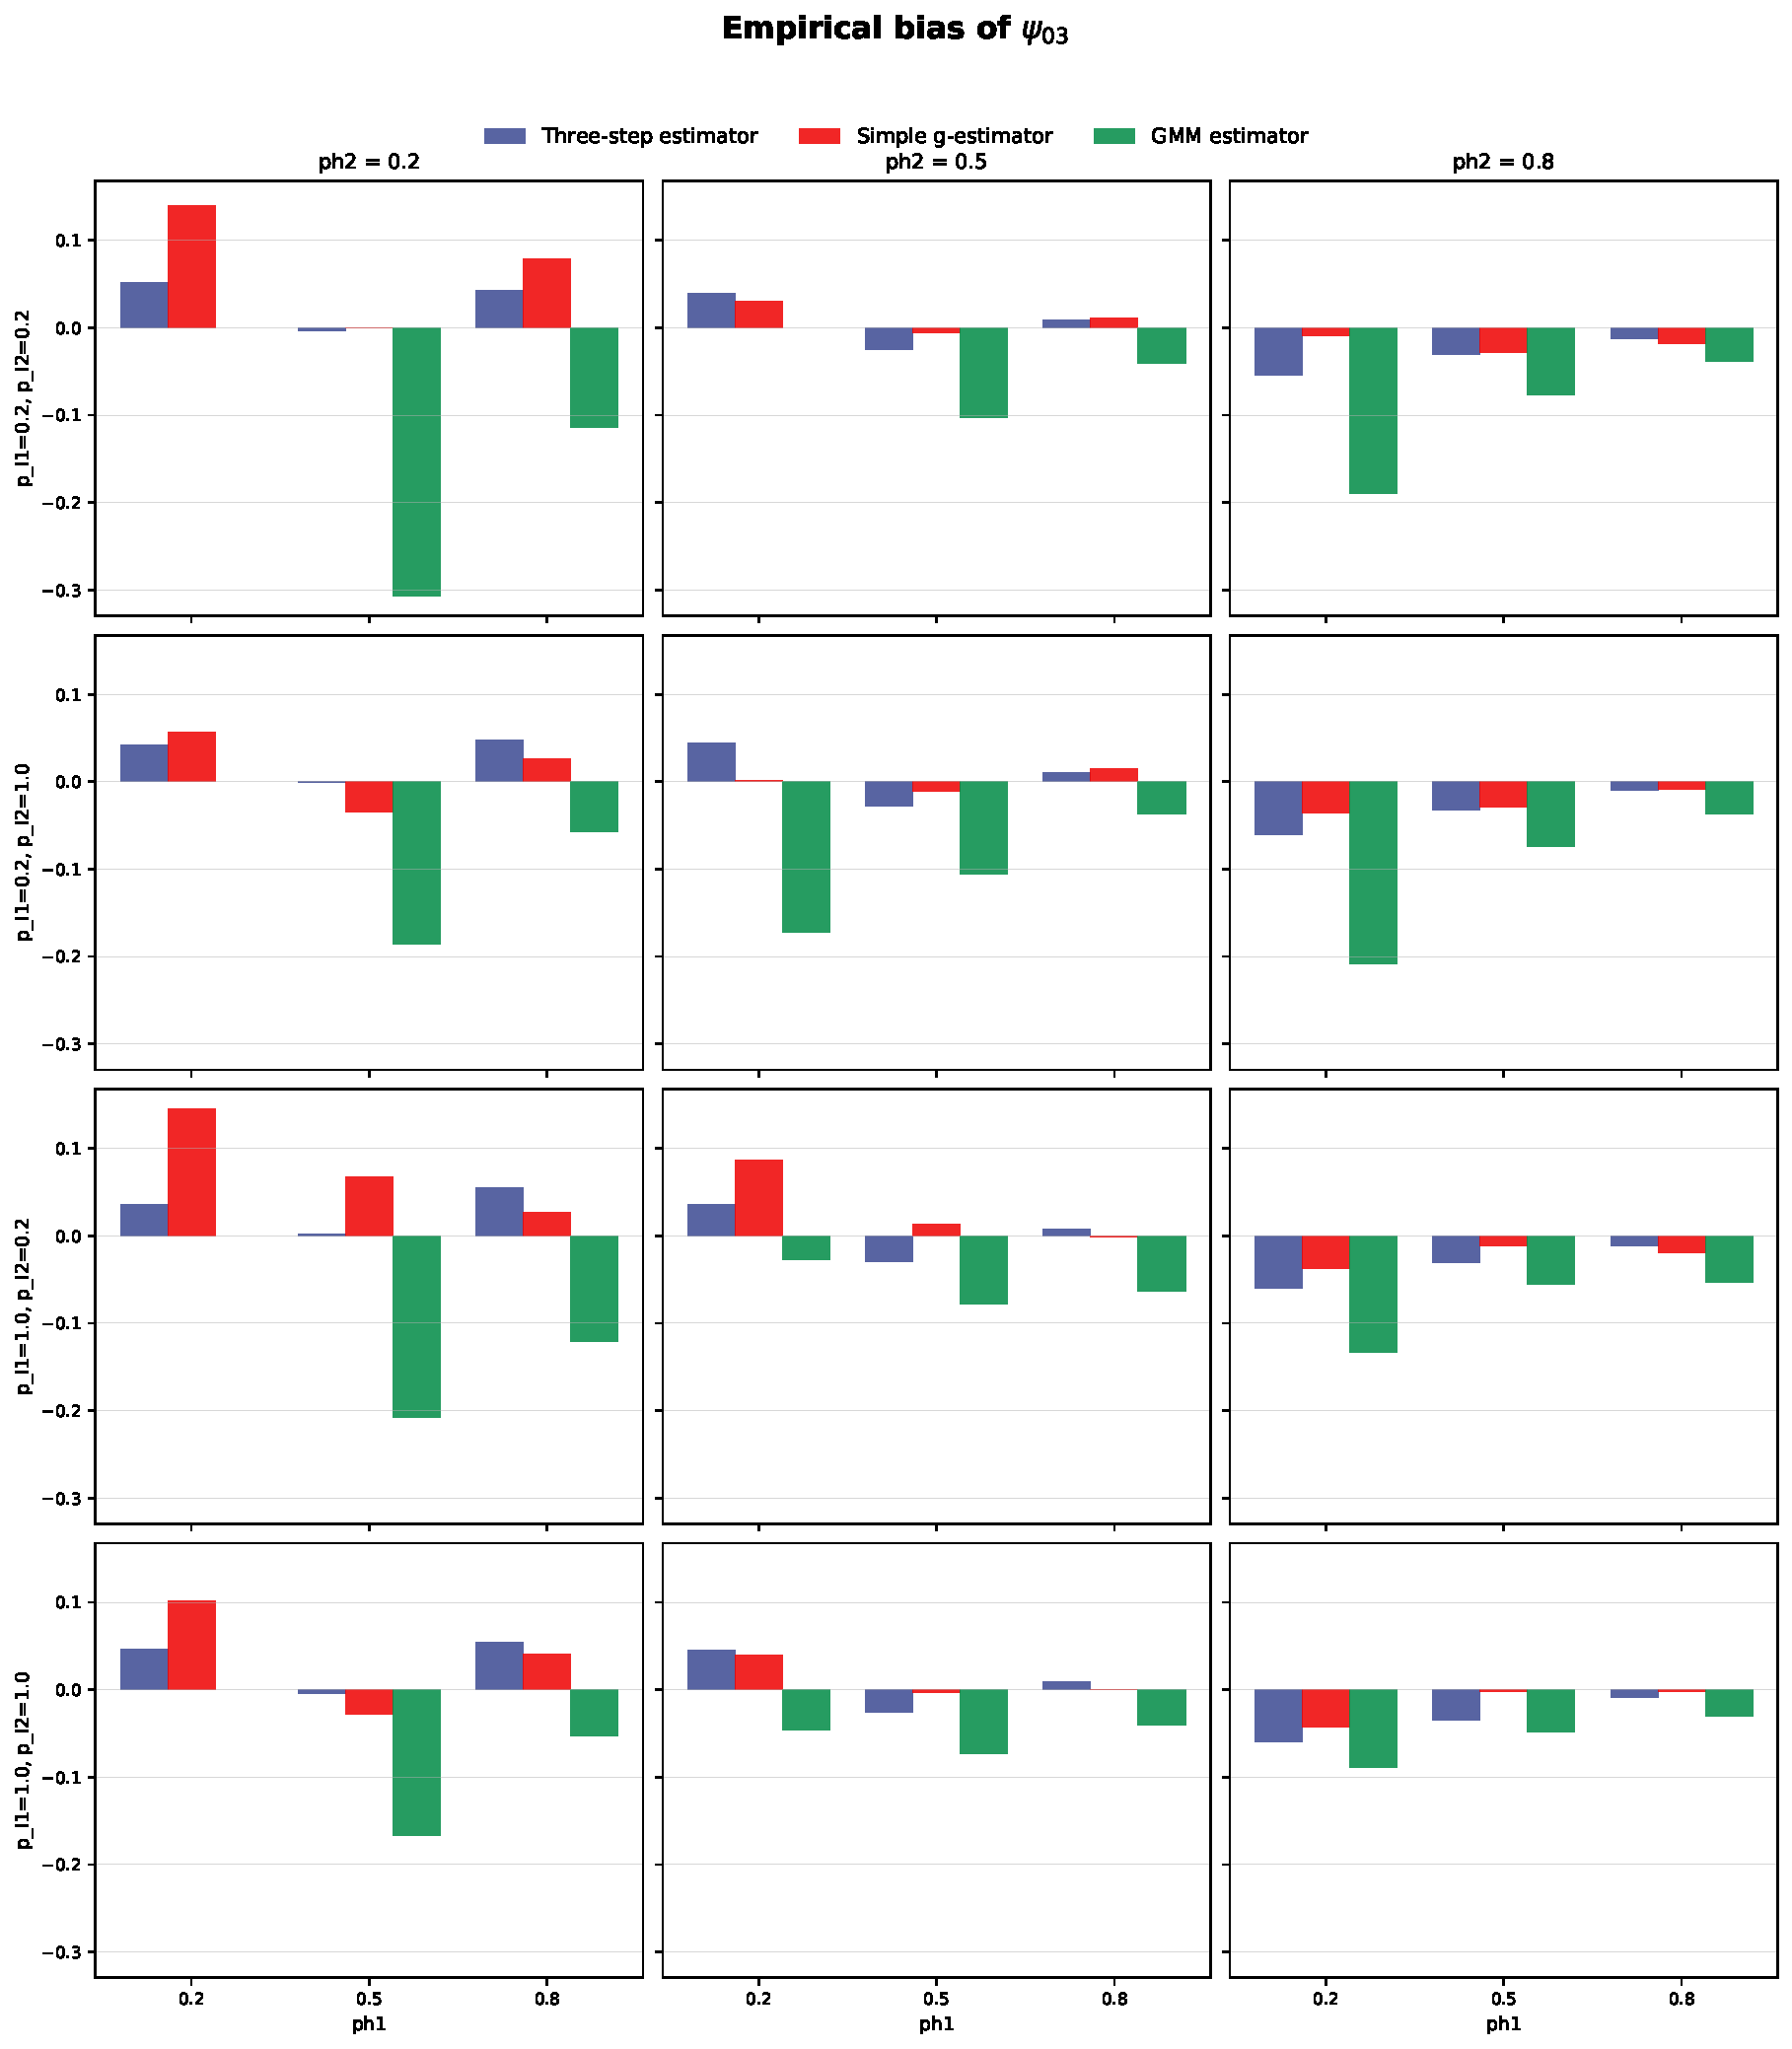
\includegraphics[width=\textwidth]{three_time_binary/psi0_python/simulation_results_plots_bias.pdf}
  \caption{S1 (null, binary DGP) --- Empirical bias of $\hat\psi_{03}$, $\hat\psi_{13}$,
           and $\hat\psi_{23}$ (rows) as a function of $p_h$ (x-axis), stratified by
           eligibility proportion $p_I$ (columns).  Grouped bars show the Three-step
           estimator (blue), Simple g-estimator (red), and GMM estimator (green).
           True values $\psi_{03}=\psi_{13}=\psi_{23}=0$.}
  \label{fig:s1_bias}
\end{figure}

\begin{figure}[htbp]
  \centering
  
\includegraphics[width=\textwidth]{three_time_binary/psi0_python/simulation_results_plots_variance.pdf}
  \caption{S1 (null, binary DGP) --- Empirical variance of $\hat\psi_{03}$, $\hat\psi_{13}$,
           and $\hat\psi_{23}$ (rows) as a function of $p_h$, stratified by $p_I$ (columns).
           Same layout as Figure~\ref{fig:s1_bias}.}
  \label{fig:s1_var}
\end{figure}

%%--------------------------------------------------------------------------
\subsection{Scenario S2: Binary Outcome, Non-null ($\psi_{03}=\psi_{13}=\psi_{23}=1$, $n=6000$)}
%%--------------------------------------------------------------------------

\begin{table}[htbp]
\centering
\caption{S2 --- Empirical bias and variance for $\hat\psi_{03}$.
         True value: $\psi_{03}=1$.}
\label{tab:s2_psi03}
\small
\begin{tabular}{cc rr rr rr}
\toprule
& & \multicolumn{2}{c}{Three-step} & \multicolumn{2}{c}{Simple g-est.} & \multicolumn{2}{c}{GMM} \\
\cmidrule(lr){3-4}\cmidrule(lr){5-6}\cmidrule(lr){7-8}
$p_h$ & $p_I$ & Bias & Var & Bias & Var & Bias & Var \\
\midrule
\multirow{4}{*}{0.4}
 & 0.25 & $\phantom{-}0.1529$ & 0.6120 & $\phantom{-}0.2427$ & 0.5465 & $\phantom{-}0.0359$ & 0.5626 \\
 & 0.50 & $\phantom{-}0.1700$ & 0.6085 & $\phantom{-}0.3033$ & 0.4548 & $\phantom{-}0.1040$ & 0.4189 \\
 & 0.75 & $\phantom{-}0.1586$ & 0.5658 & $\phantom{-}0.2376$ & 0.3231 & $\phantom{-}0.0993$ & 0.3335 \\
 & 1.00 & $\phantom{-}0.1693$ & 0.5769 & $\phantom{-}0.0935$ & 0.1924 & $\phantom{-}0.0231$ & 0.1974 \\
\midrule
\multirow{4}{*}{0.6}
 & 0.25 & $-0.0161$ & 0.2272 & $\phantom{-}0.0762$ & 0.2068 & $-0.0318$ & 0.2131 \\
 & 0.50 & $-0.0166$ & 0.2210 & $\phantom{-}0.1190$ & 0.1885 & $-0.0016$ & 0.1943 \\
 & 0.75 & $-0.0127$ & 0.2214 & $\phantom{-}0.0916$ & 0.1864 & $\phantom{-}0.0278$ & 0.1831 \\
 & 1.00 & $-0.0114$ & 0.2240 & $\phantom{-}0.0526$ & 0.1414 & $\phantom{-}0.0037$ & 0.1339 \\
\midrule
\multirow{4}{*}{0.8}
 & 0.25 & $-0.0019$ & 0.0973 & $\phantom{-}0.0385$ & 0.0916 & $-0.0164$ & 0.0920 \\
 & 0.50 & $-0.0032$ & 0.0971 & $\phantom{-}0.0568$ & 0.0925 & $\phantom{-}0.0045$ & 0.0934 \\
 & 0.75 & $-0.0032$ & 0.0974 & $\phantom{-}0.0487$ & 0.0936 & $\phantom{-}0.0093$ & 0.0942 \\
 & 1.00 & $-0.0027$ & 0.0952 & $\phantom{-}0.0282$ & 0.0789 & $-0.0003$ & 0.0777 \\
\bottomrule
\end{tabular}
\end{table}

\begin{table}[htbp]
\centering
\caption{S2 --- Empirical bias and variance for $\hat\psi_{13}$.
         True value: $\psi_{13}=1$.}
\label{tab:s2_psi13}
\small
\begin{tabular}{cc rr rr rr}
\toprule
& & \multicolumn{2}{c}{Three-step} & \multicolumn{2}{c}{Simple g-est.} & \multicolumn{2}{c}{GMM} \\
\cmidrule(lr){3-4}\cmidrule(lr){5-6}\cmidrule(lr){7-8}
$p_h$ & $p_I$ & Bias & Var & Bias & Var & Bias & Var \\
\midrule
\multirow{4}{*}{0.4}
 & 0.25 & $\phantom{-}0.2780$ & 0.4177 & $\phantom{-}0.2461$ & 0.3830 & $\phantom{-}0.2161$ & 0.4209 \\
 & 0.50 & $\phantom{-}0.2351$ & 0.1832 & $\phantom{-}0.2020$ & 0.1374 & $\phantom{-}0.1483$ & 0.1500 \\
 & 0.75 & $\phantom{-}0.1510$ & 0.1069 & $\phantom{-}0.1127$ & 0.0983 & $\phantom{-}0.0639$ & 0.0999 \\
 & 1.00 & $\phantom{-}0.0566$ & 0.0767 & $\phantom{-}0.0396$ & 0.0696 & $\phantom{-}0.0015$ & 0.0747 \\
\midrule
\multirow{4}{*}{0.6}
 & 0.25 & $\phantom{-}0.2528$ & 0.3428 & $\phantom{-}0.2420$ & 0.3081 & $\phantom{-}0.1763$ & 0.2951 \\
 & 0.50 & $\phantom{-}0.1896$ & 0.1900 & $\phantom{-}0.1631$ & 0.1677 & $\phantom{-}0.1038$ & 0.1638 \\
 & 0.75 & $\phantom{-}0.0936$ & 0.0788 & $\phantom{-}0.0762$ & 0.0728 & $\phantom{-}0.0492$ & 0.0684 \\
 & 1.00 & $\phantom{-}0.0269$ & 0.0782 & $\phantom{-}0.0202$ & 0.0727 & $\phantom{-}0.0010$ & 0.0685 \\
\midrule
\multirow{4}{*}{0.8}
 & 0.25 & $\phantom{-}0.2077$ & 0.3600 & $\phantom{-}0.2117$ & 0.3316 & $\phantom{-}0.1110$ & 0.3016 \\
 & 0.50 & $\phantom{-}0.1728$ & 0.1373 & $\phantom{-}0.1610$ & 0.1453 & $\phantom{-}0.0932$ & 0.1336 \\
 & 0.75 & $\phantom{-}0.1095$ & 0.0945 & $\phantom{-}0.0852$ & 0.0875 & $\phantom{-}0.0422$ & 0.0804 \\
 & 1.00 & $\phantom{-}0.0365$ & 0.0626 & $\phantom{-}0.0222$ & 0.0592 & $-0.0018$ & 0.0560 \\
\bottomrule
\end{tabular}
\end{table}

\begin{table}[htbp]
\centering
\caption{S2 --- Empirical bias and variance for $\hat\psi_{23}$.
         True value: $\psi_{23}=1$.
         TS and SG are identical for $\hat\psi_{23}$ by construction.}
\label{tab:s2_psi23}
\small
\begin{tabular}{cc rr rr rr}
\toprule
& & \multicolumn{2}{c}{Three-step} & \multicolumn{2}{c}{Simple g-est.} & \multicolumn{2}{c}{GMM} \\
\cmidrule(lr){3-4}\cmidrule(lr){5-6}\cmidrule(lr){7-8}
$p_h$ & $p_I$ & Bias & Var & Bias & Var & Bias & Var \\
\midrule
\multirow{4}{*}{0.4}
 & 0.25 & $-0.0241$ & 0.1636 & $-0.0241$ & 0.1636 & $-0.0335$ & 0.1705 \\
 & 0.50 & $\phantom{-}0.0115$ & 0.0583 & $\phantom{-}0.0115$ & 0.0583 & $-0.0044$ & 0.0603 \\
 & 0.75 & $\phantom{-}0.0148$ & 0.0465 & $\phantom{-}0.0148$ & 0.0465 & $-0.0049$ & 0.0471 \\
 & 1.00 & $\phantom{-}0.0024$ & 0.0333 & $\phantom{-}0.0024$ & 0.0333 & $-0.0140$ & 0.0331 \\
\midrule
\multirow{4}{*}{0.6}
 & 0.25 & $\phantom{-}0.0223$ & 0.1078 & $\phantom{-}0.0223$ & 0.1078 & $\phantom{-}0.0078$ & 0.1043 \\
 & 0.50 & $\phantom{-}0.0108$ & 0.0606 & $\phantom{-}0.0108$ & 0.0606 & $-0.0155$ & 0.0558 \\
 & 0.75 & $-0.0012$ & 0.0511 & $-0.0012$ & 0.0511 & $-0.0136$ & 0.0511 \\
 & 1.00 & $\phantom{-}0.0058$ & 0.0414 & $\phantom{-}0.0058$ & 0.0414 & $-0.0007$ & 0.0398 \\
\midrule
\multirow{4}{*}{0.8}
 & 0.25 & $\phantom{-}0.0313$ & 0.2726 & $\phantom{-}0.0313$ & 0.2726 & $-0.0090$ & 0.2136 \\
 & 0.50 & $\phantom{-}0.0409$ & 0.1090 & $\phantom{-}0.0409$ & 0.1090 & $\phantom{-}0.0297$ & 0.1070 \\
 & 0.75 & $\phantom{-}0.0206$ & 0.0666 & $\phantom{-}0.0206$ & 0.0666 & $\phantom{-}0.0157$ & 0.0666 \\
 & 1.00 & $\phantom{-}0.0183$ & 0.0563 & $\phantom{-}0.0183$ & 0.0563 & $\phantom{-}0.0143$ & 0.0539 \\
\bottomrule
\end{tabular}
\end{table}

\begin{figure}[htbp]
  \centering
  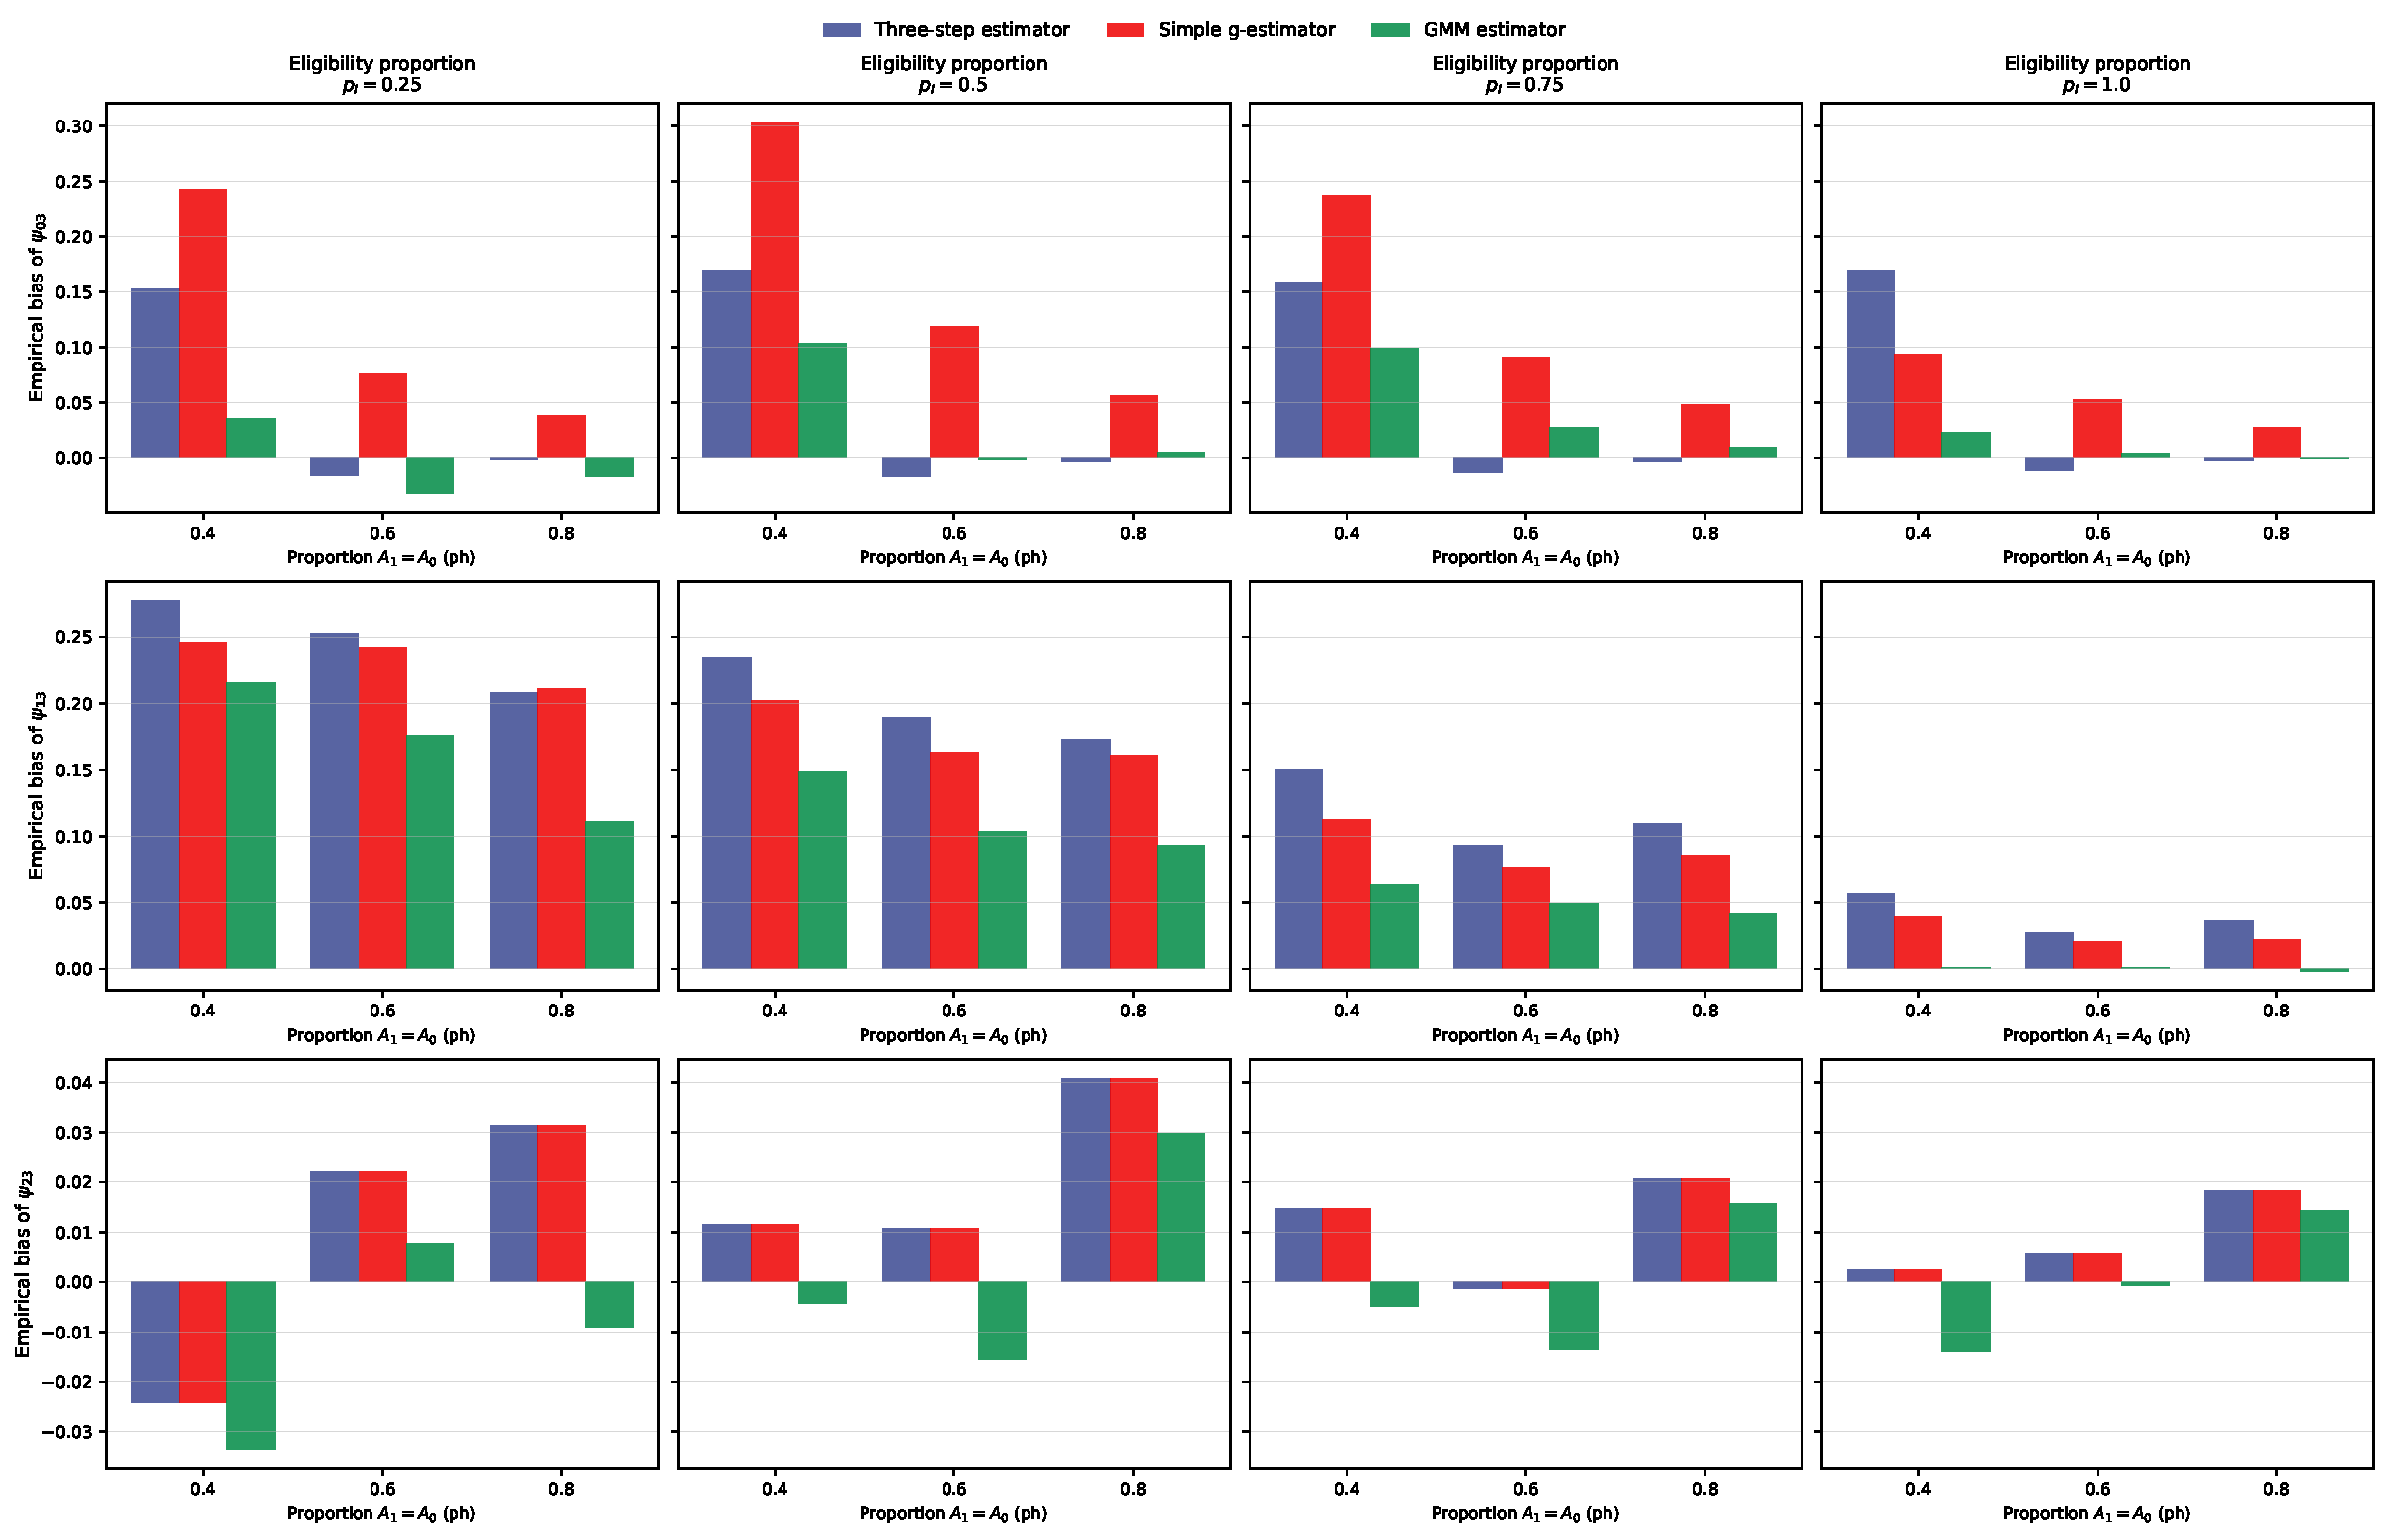
\includegraphics[width=\textwidth]{three_time_binary/psi1_python/simulation_results_plots_bias.pdf}
  \caption{S2 (binary DGP, $\psi=1$) --- Empirical bias of $\hat\psi_{03}$, $\hat\psi_{13}$,
           and $\hat\psi_{23}$ (rows) as a function of $p_h$, stratified by $p_I$ (columns).
           True values $\psi_{03}=\psi_{13}=\psi_{23}=1$.}
  \label{fig:s2_bias}
\end{figure}

\begin{figure}[htbp]
  \centering
  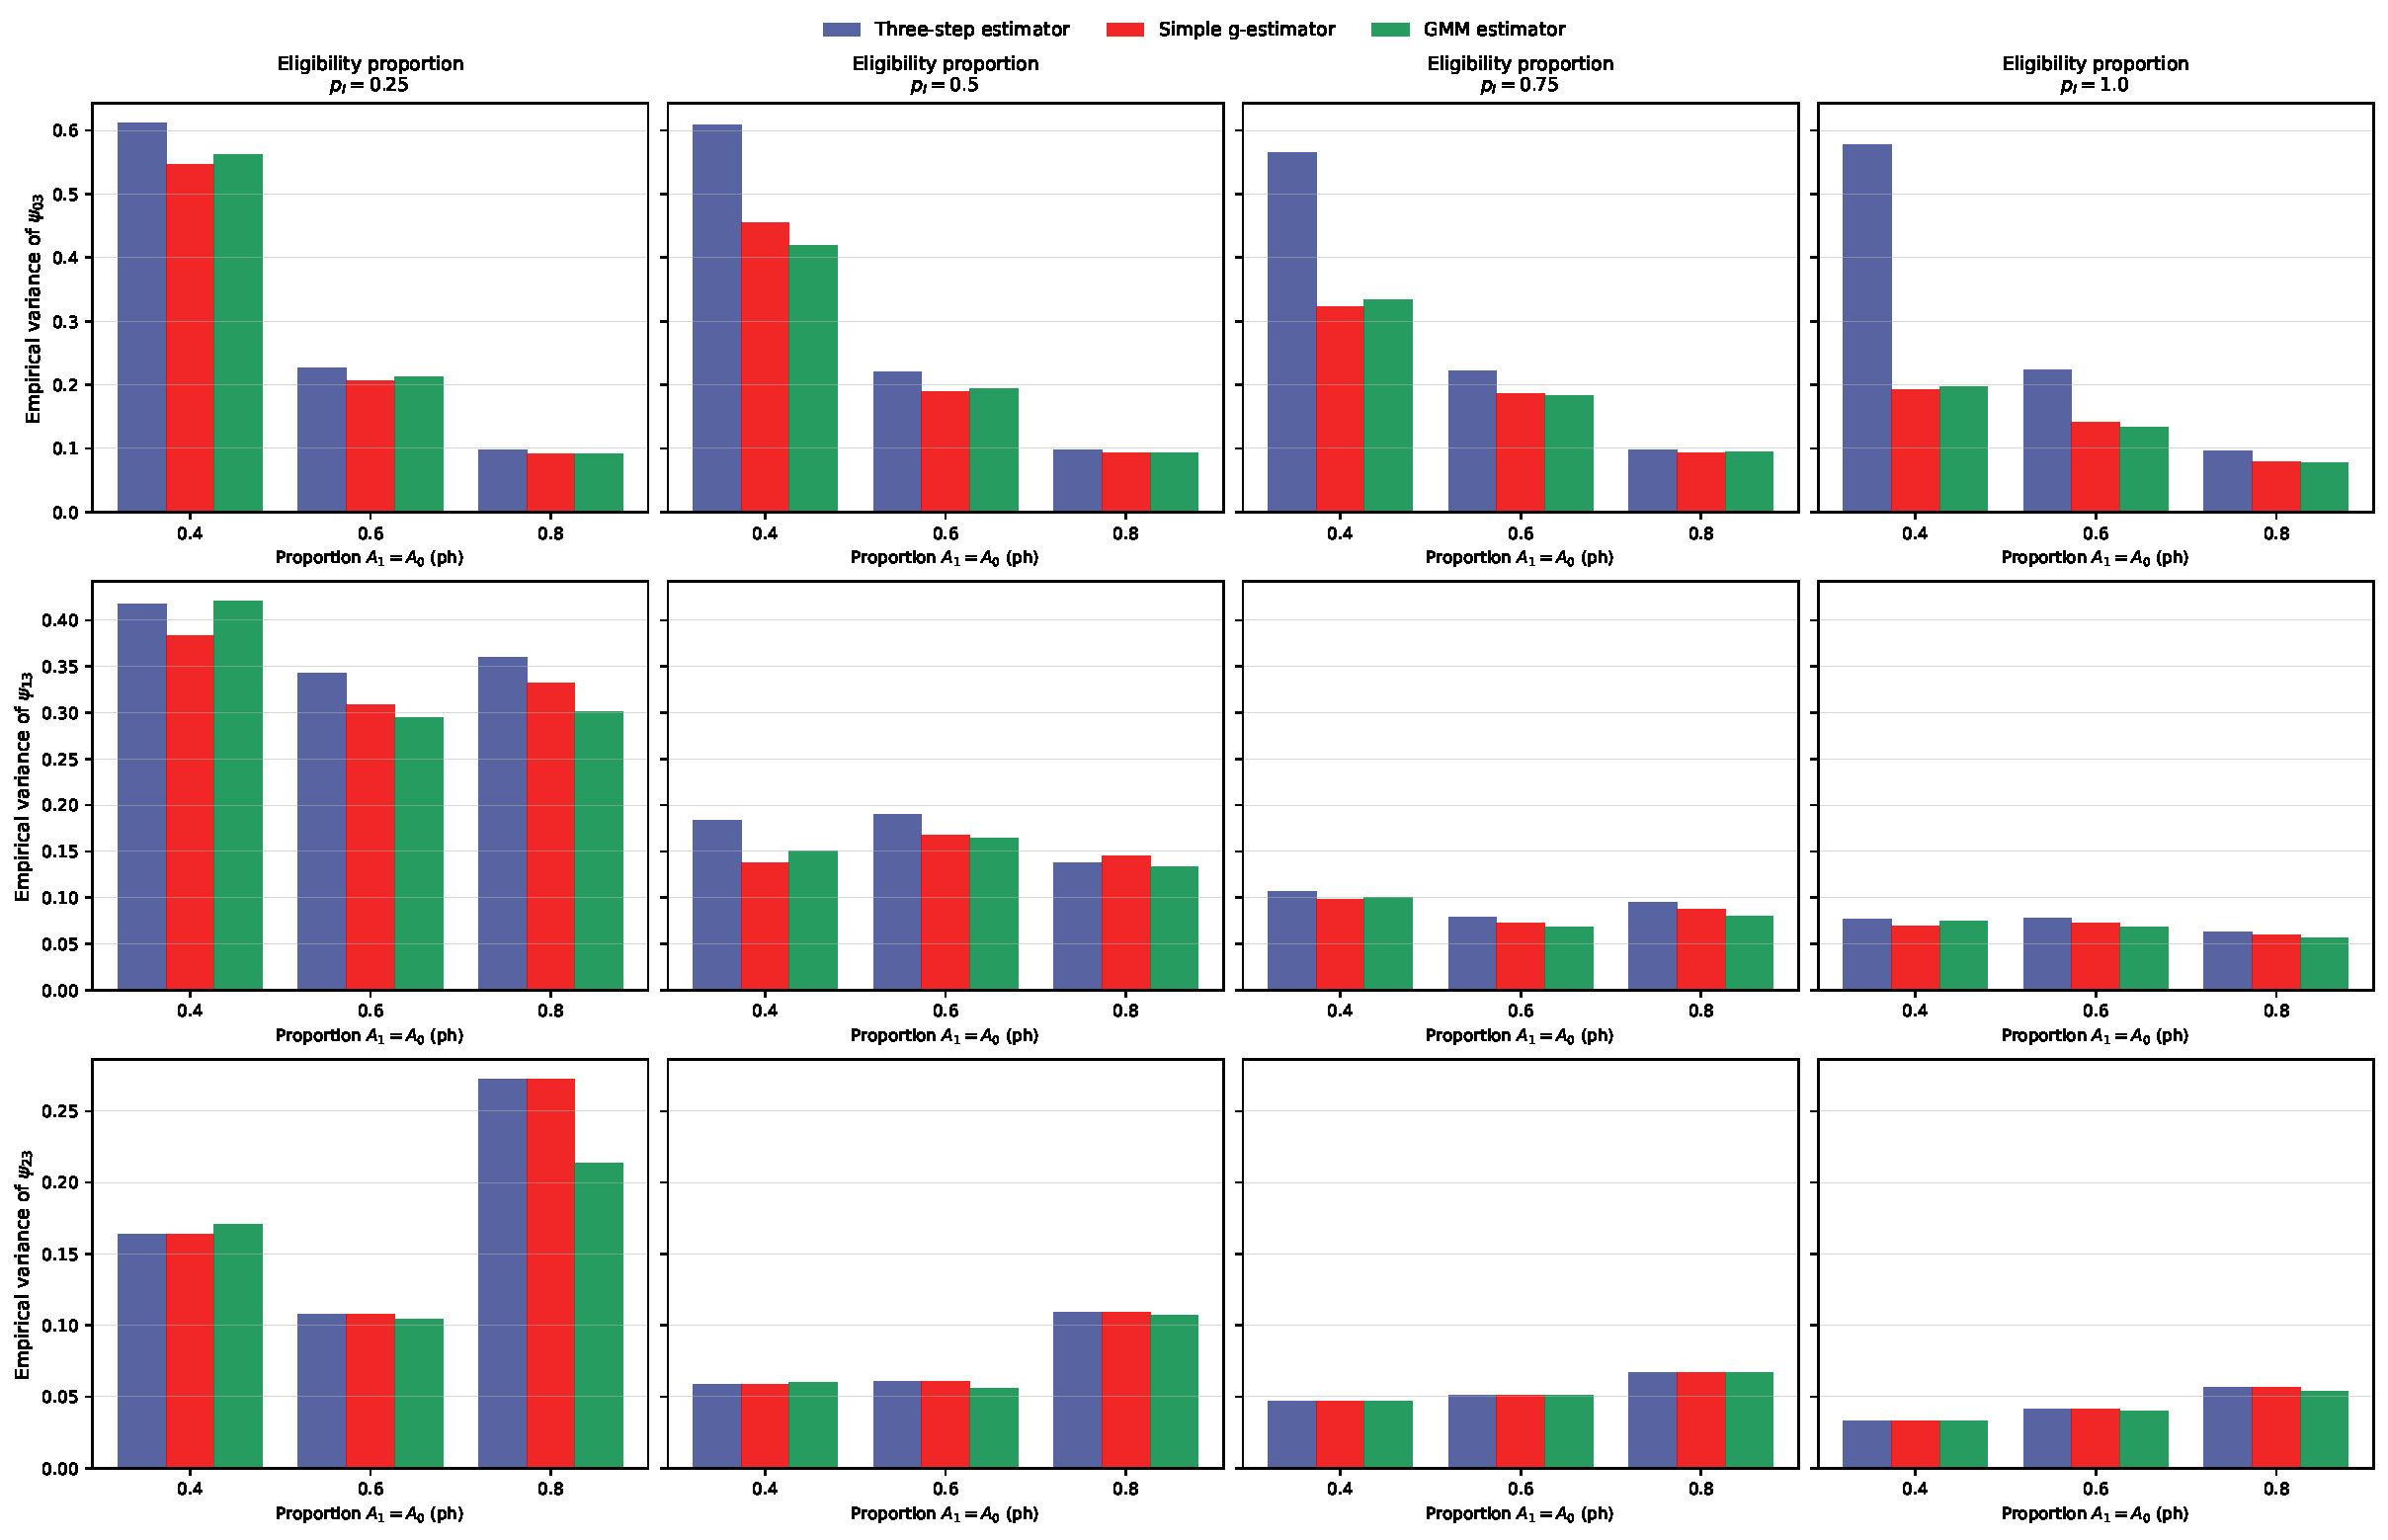
\includegraphics[width=\textwidth]{three_time_binary/psi1_python/simulation_results_plots_variance.pdf}
  \caption{S2 (binary DGP, $\psi=1$) --- Empirical variance of $\hat\psi_{03}$, $\hat\psi_{13}$,
           and $\hat\psi_{23}$ (rows) as a function of $p_h$, stratified by $p_I$ (columns).}
  \label{fig:s2_var}
\end{figure}

%%--------------------------------------------------------------------------
\subsection{Scenario S3: Continuous Outcome, $\sigma=0$ ($\psi=1$, $n=4000$)}
%%--------------------------------------------------------------------------

When $\sigma=0$, the outcome is deterministic given the treatment and
covariate history (variance of $Y$ equals 1 regardless of treatment,
since $\sigma_Y=0\cdot(\cdots)+1=1$; in practice $\sigma=0$ collapses
the noise to its floor).  All three estimators recover the true parameters
with negligible Monte Carlo bias ($|\mathrm{Bias}|<5\times10^{-4}$) and
near-zero variance ($<10^{-6}$) across all 12 $(p_h,\,p_I)$ cells.
No numerical table is presented, but the corresponding plots are shown in
Figures~\ref{fig:s3_bias} and~\ref{fig:s3_var} to confirm the near-zero
performance visually.

\begin{figure}[htbp]
  \centering
  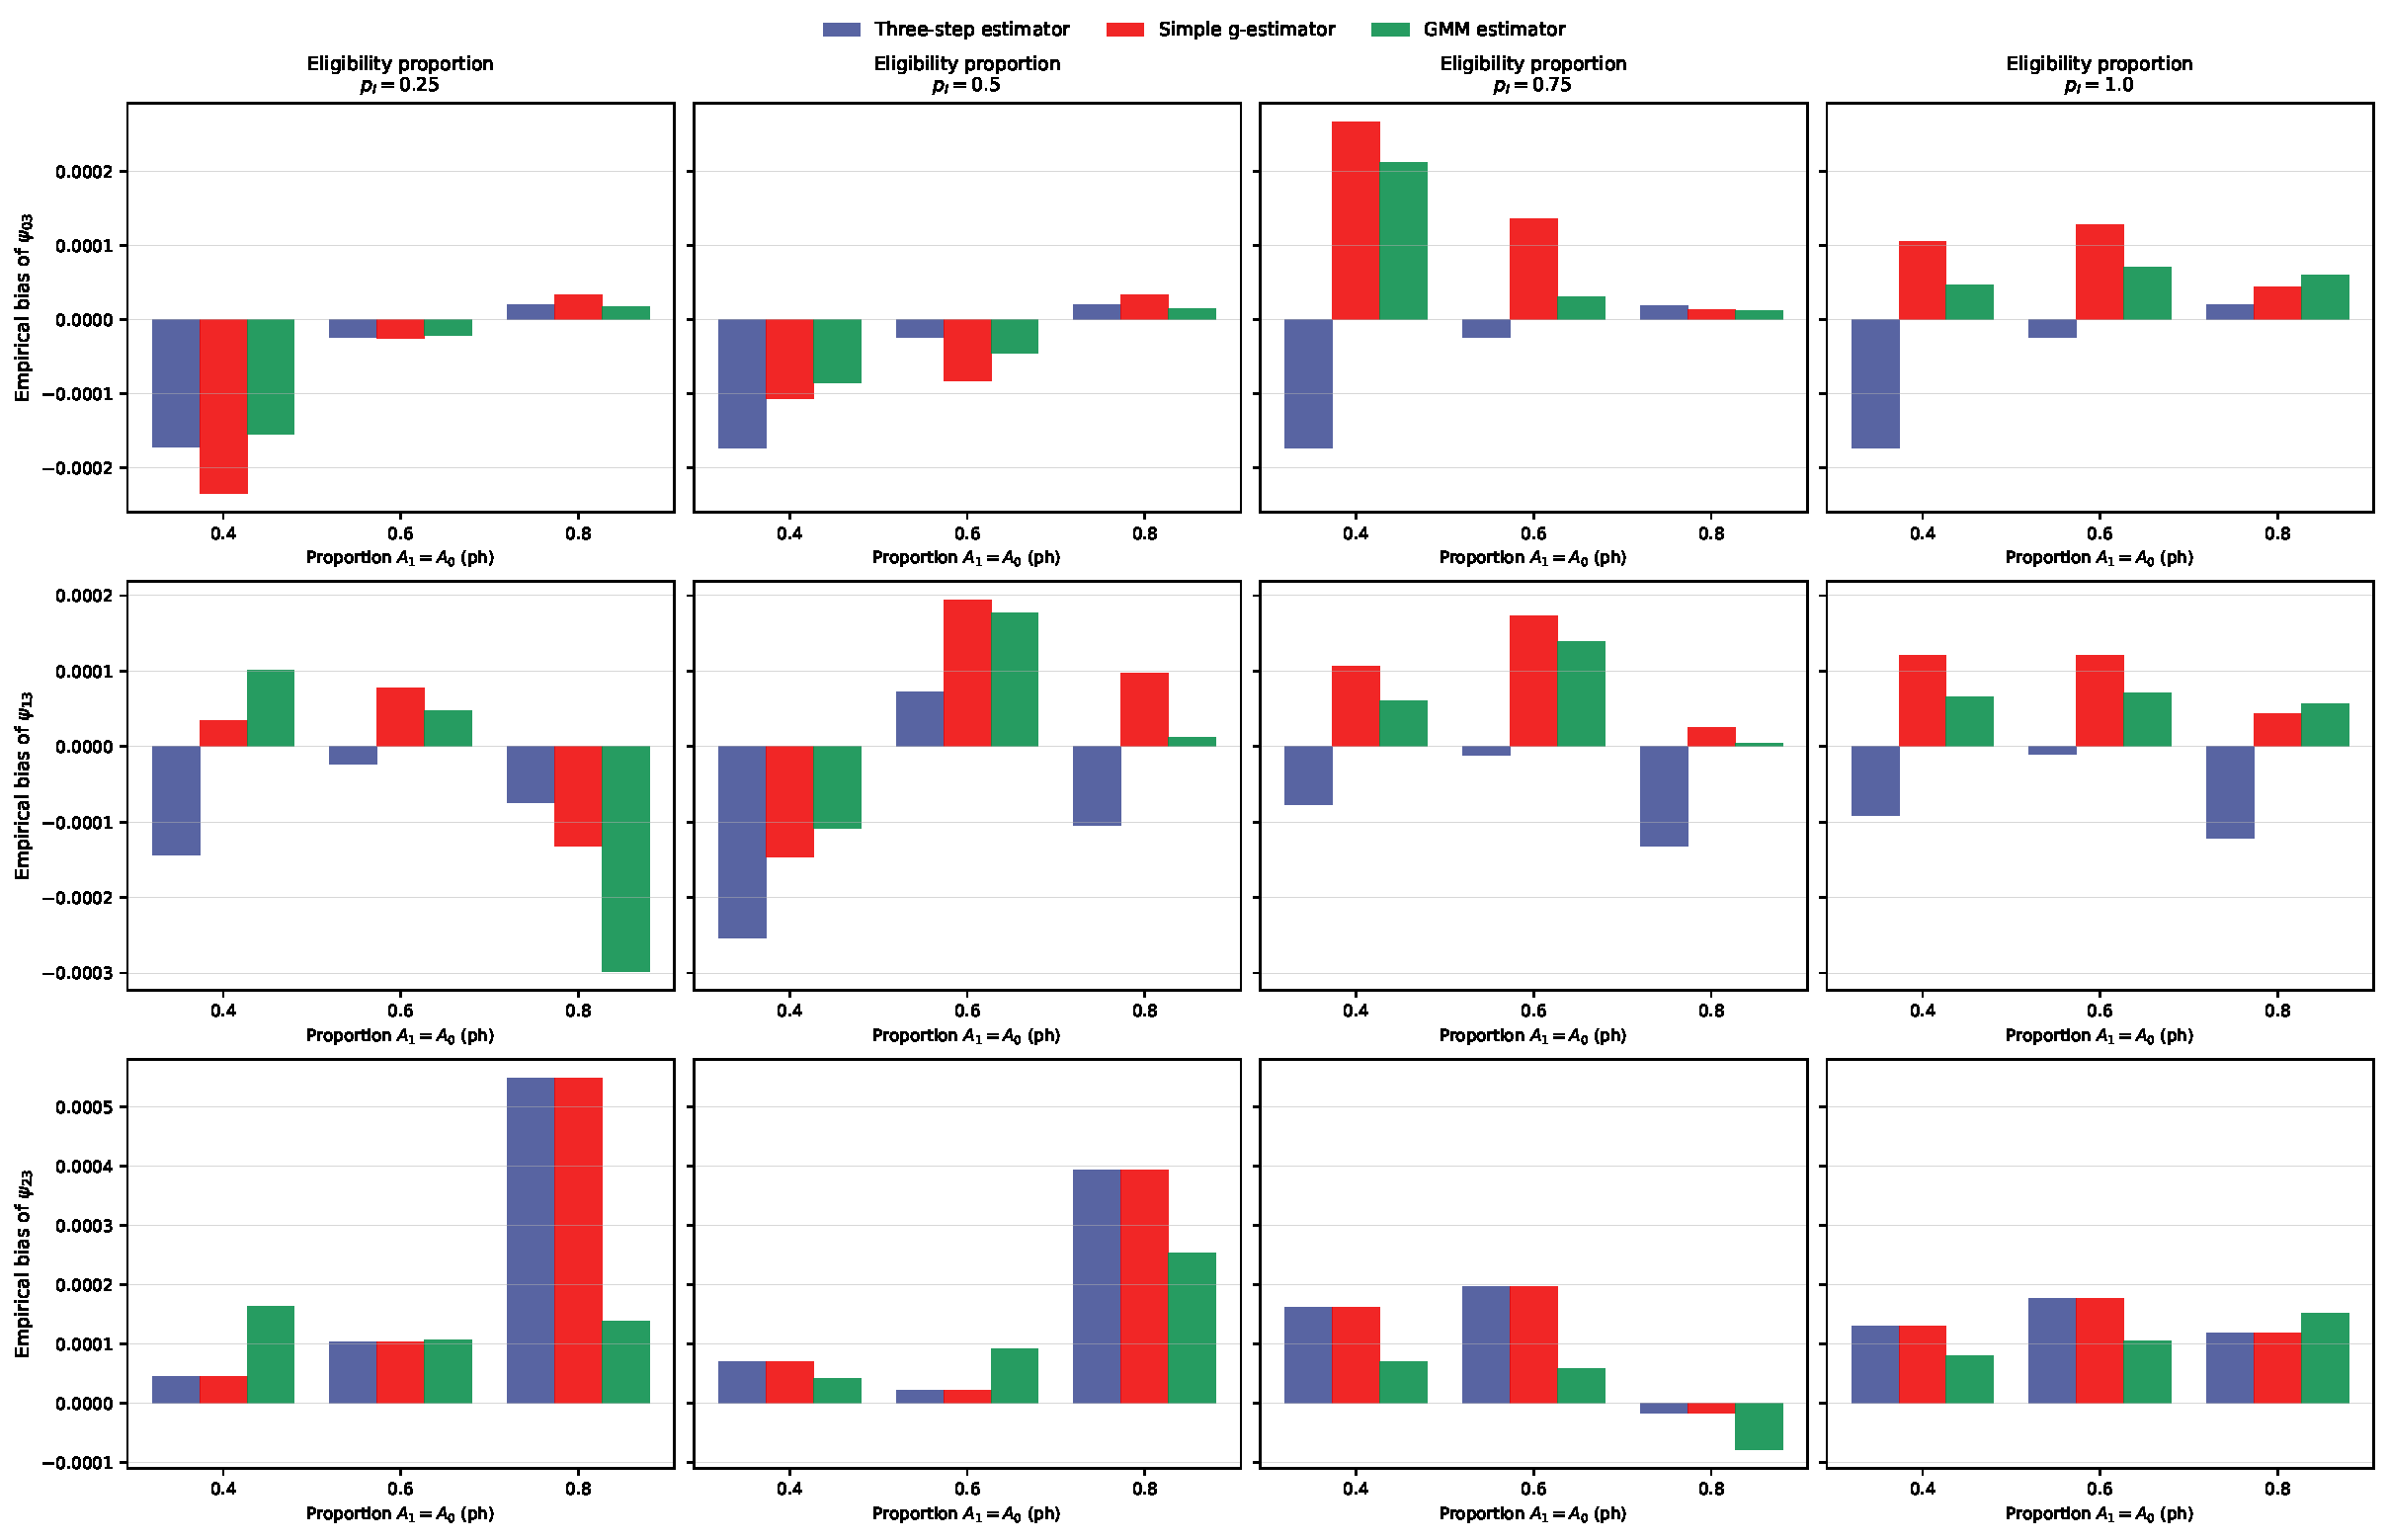
\includegraphics[width=\textwidth]{three_time_continuous/psi1_python/simulation_results_plots_bias.pdf}
  \caption{S3 (continuous DGP, $\sigma=0$, $\psi=1$) --- Empirical bias of
           $\hat\psi_{03}$, $\hat\psi_{13}$, and $\hat\psi_{23}$ (rows) as a function
           of $p_h$, stratified by $p_I$ (columns).  All biases are negligibly small
           ($<5\times10^{-4}$), confirming perfect identification in the deterministic case.}
  \label{fig:s3_bias}
\end{figure}

\begin{figure}[htbp]
  \centering
  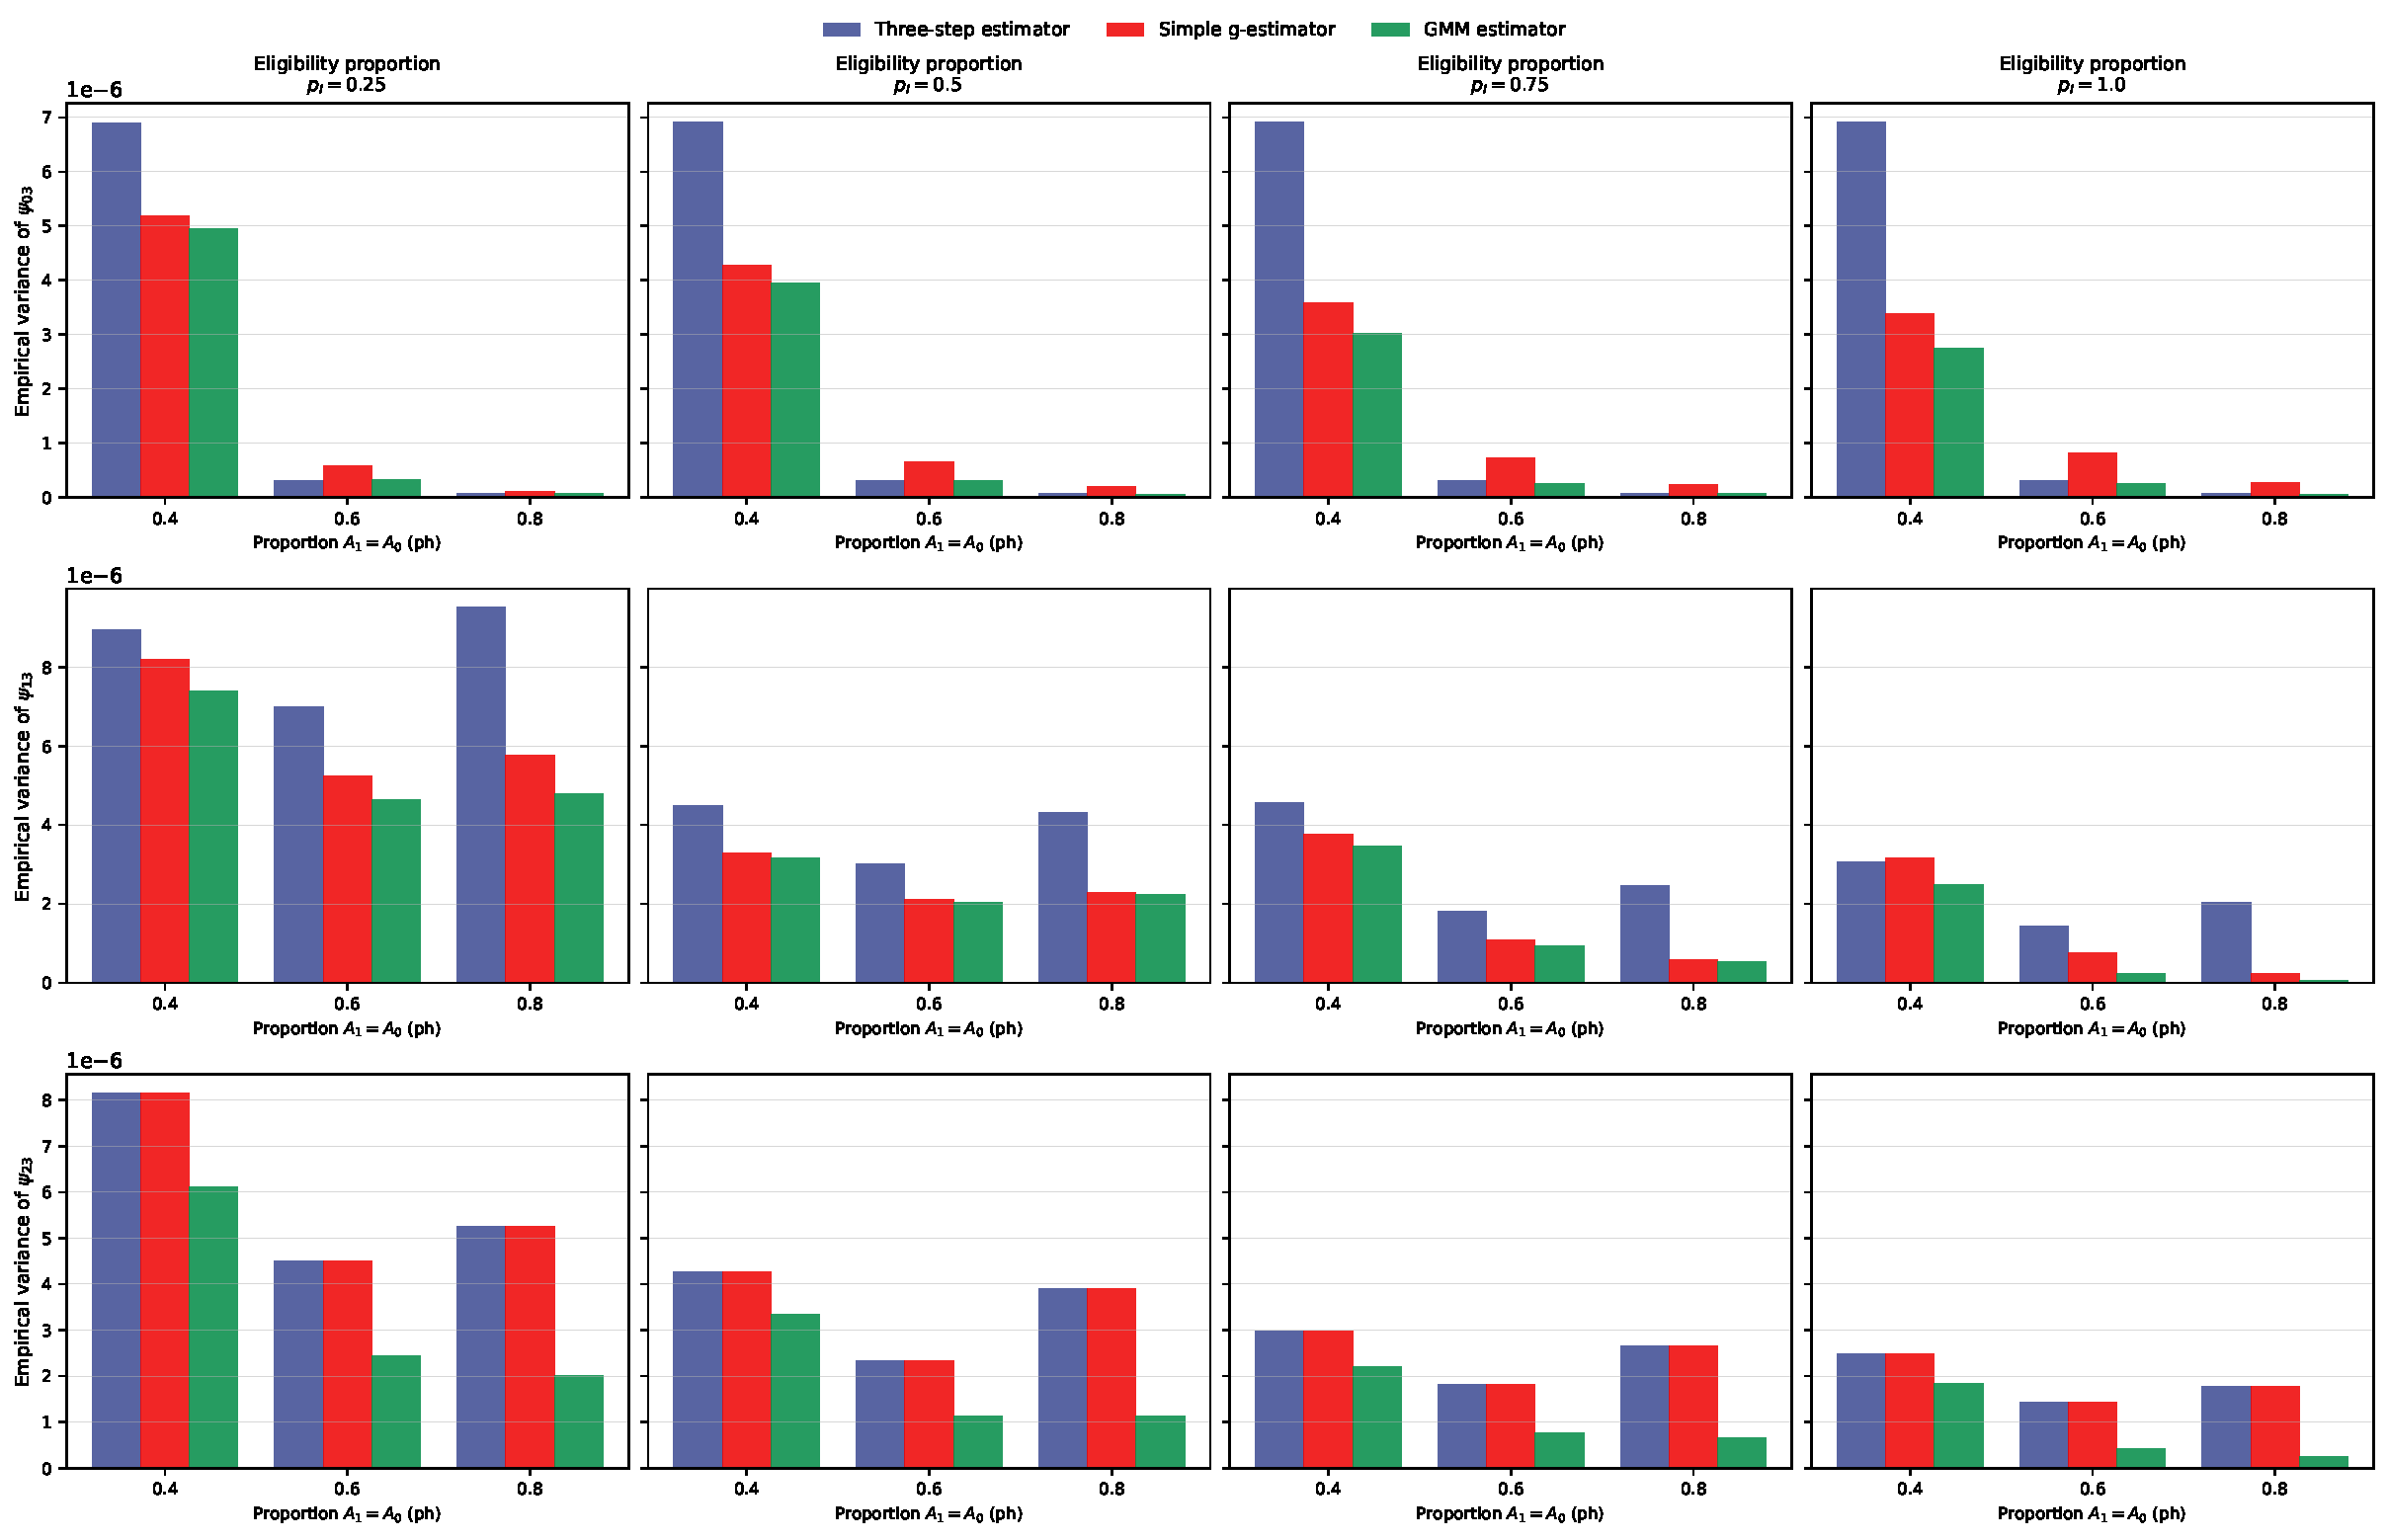
\includegraphics[width=\textwidth]{three_time_continuous/psi1_python/simulation_results_plots_variance.pdf}
  \caption{S3 (continuous DGP, $\sigma=0$, $\psi=1$) --- Empirical variance of
           $\hat\psi_{03}$, $\hat\psi_{13}$, and $\hat\psi_{23}$ (rows) as a function
           of $p_h$, stratified by $p_I$ (columns).  Variances are effectively zero
           throughout.}
  \label{fig:s3_var}
\end{figure}

%%--------------------------------------------------------------------------
\subsection{Scenario S4: Continuous Outcome, $\sigma=10$ ($\psi=1$, $n=4000$)}
%%--------------------------------------------------------------------------

\begin{table}[htbp]
\centering
\caption{S4 ($\sigma=10$) --- Empirical bias and variance for $\hat\psi_{03}$.
         True value: $\psi_{03}=1$.}
\label{tab:s4_psi03}
\small
\begin{tabular}{cc rr rr rr}
\toprule
& & \multicolumn{2}{c}{Three-step} & \multicolumn{2}{c}{Simple g-est.} & \multicolumn{2}{c}{GMM} \\
\cmidrule(lr){3-4}\cmidrule(lr){5-6}\cmidrule(lr){7-8}
$p_h$ & $p_I$ & Bias & Var & Bias & Var & Bias & Var \\
\midrule
\multirow{4}{*}{0.4}
 & 0.25 & $-0.5996$ & 22.67 & $-0.6513$ & 18.65 & $-0.6628$ & 18.23 \\
 & 0.50 & $-0.6011$ & 22.59 & $-0.3791$ & 16.17 & $-0.3445$ & 15.75 \\
 & 0.75 & $-0.5907$ & 22.70 & $-0.2159$ & 19.33 & $-0.3146$ & 17.28 \\
 & 1.00 & $-0.6016$ & 22.66 & $-0.1857$ & 16.24 & $-0.2043$ & 13.64 \\
\midrule
\multirow{4}{*}{0.6}
 & 0.25 & $\phantom{-}0.0431$ & 5.353 & $-0.1727$ & 5.779 & $-0.0709$ & 5.225 \\
 & 0.50 & $\phantom{-}0.0444$ & 5.345 & $-0.2589$ & 6.758 & $-0.1207$ & 5.272 \\
 & 0.75 & $\phantom{-}0.0424$ & 5.340 & $-0.1095$ & 5.466 & $-0.0142$ & 4.166 \\
 & 1.00 & $\phantom{-}0.0448$ & 5.349 & $-0.2782$ & 6.126 & $-0.0973$ & 4.219 \\
\midrule
\multirow{4}{*}{0.8}
 & 0.25 & $\phantom{-}0.2160$ & 3.012 & $\phantom{-}0.0533$ & 3.270 & $\phantom{-}0.1183$ & 3.059 \\
 & 0.50 & $\phantom{-}0.2166$ & 3.017 & $-0.0012$ & 3.611 & $\phantom{-}0.1026$ & 3.224 \\
 & 0.75 & $\phantom{-}0.2156$ & 3.012 & $\phantom{-}0.0395$ & 3.336 & $\phantom{-}0.1329$ & 2.963 \\
 & 1.00 & $\phantom{-}0.2144$ & 3.011 & $-0.1251$ & 3.510 & $\phantom{-}0.0352$ & 2.899 \\
\bottomrule
\end{tabular}
\end{table}

\begin{table}[htbp]
\centering
\caption{S4 ($\sigma=10$) --- Empirical bias and variance for $\hat\psi_{13}$.
         True value: $\psi_{13}=1$.}
\label{tab:s4_psi13}
\small
\begin{tabular}{cc rr rr rr}
\toprule
& & \multicolumn{2}{c}{Three-step} & \multicolumn{2}{c}{Simple g-est.} & \multicolumn{2}{c}{GMM} \\
\cmidrule(lr){3-4}\cmidrule(lr){5-6}\cmidrule(lr){7-8}
$p_h$ & $p_I$ & Bias & Var & Bias & Var & Bias & Var \\
\midrule
\multirow{4}{*}{0.4}
 & 0.25 & $-0.3837$ & 21.85 & $-0.2658$ & 20.35 & $-0.3328$ & 18.42 \\
 & 0.50 & $-0.1468$ & 11.32 & $-0.0535$ & 12.31 & $-0.0320$ & 11.60 \\
 & 0.75 & $\phantom{-}0.0825$ & 6.975 & $\phantom{-}0.3096$ & 6.752 & $\phantom{-}0.2619$ & 6.276 \\
 & 1.00 & $-0.0355$ & 5.028 & $-0.0354$ & 5.877 & $-0.0049$ & 5.186 \\
\midrule
\multirow{4}{*}{0.6}
 & 0.25 & $\phantom{-}0.5737$ & 16.83 & $\phantom{-}0.5711$ & 15.32 & $\phantom{-}0.4188$ & 15.39 \\
 & 0.50 & $\phantom{-}0.2601$ & 7.104 & $\phantom{-}0.2034$ & 6.145 & $\phantom{-}0.1475$ & 5.631 \\
 & 0.75 & $-0.3680$ & 4.896 & $-0.1316$ & 4.163 & $-0.2394$ & 3.737 \\
 & 1.00 & $-0.1374$ & 3.428 & $-0.0665$ & 2.947 & $-0.0832$ & 2.864 \\
\midrule
\multirow{4}{*}{0.8}
 & 0.25 & $\phantom{-}0.3993$ & 25.31 & $\phantom{-}0.5403$ & 24.42 & $\phantom{-}0.2882$ & 18.74 \\
 & 0.50 & $\phantom{-}0.0845$ & 9.281 & $\phantom{-}0.2481$ & 9.398 & $\phantom{-}0.0360$ & 7.150 \\
 & 0.75 & $-0.1501$ & 7.008 & $\phantom{-}0.0322$ & 6.429 & $-0.1155$ & 5.791 \\
 & 1.00 & $-0.0200$ & 4.976 & $\phantom{-}0.1700$ & 4.548 & $-0.0873$ & 4.152 \\
\bottomrule
\end{tabular}
\end{table}

\begin{table}[htbp]
\centering
\caption{S4 ($\sigma=10$) --- Empirical bias and variance for $\hat\psi_{23}$.
         True value: $\psi_{23}=1$.
         TS and SG are identical for $\hat\psi_{23}$ by construction.}
\label{tab:s4_psi23}
\small
\begin{tabular}{cc rr rr rr}
\toprule
& & \multicolumn{2}{c}{Three-step} & \multicolumn{2}{c}{Simple g-est.} & \multicolumn{2}{c}{GMM} \\
\cmidrule(lr){3-4}\cmidrule(lr){5-6}\cmidrule(lr){7-8}
$p_h$ & $p_I$ & Bias & Var & Bias & Var & Bias & Var \\
\midrule
\multirow{4}{*}{0.4}
 & 0.25 & $-0.2702$ & 22.98 & $-0.2702$ & 22.98 & $-0.3021$ & 20.16 \\
 & 0.50 & $-0.1779$ & 11.43 & $-0.1779$ & 11.43 & $-0.1924$ & 11.30 \\
 & 0.75 & $\phantom{-}0.0480$ & 6.578 & $\phantom{-}0.0480$ & 6.578 & $-0.0371$ & 6.056 \\
 & 1.00 & $-0.0356$ & 6.109 & $-0.0356$ & 6.109 & $-0.0588$ & 5.322 \\
\midrule
\multirow{4}{*}{0.6}
 & 0.25 & $-0.3833$ & 24.64 & $-0.3833$ & 24.64 & $-0.3055$ & 23.08 \\
 & 0.50 & $-0.2833$ & 10.61 & $-0.2833$ & 10.61 & $-0.2416$ & 9.770 \\
 & 0.75 & $-0.0291$ & 4.912 & $-0.0291$ & 4.912 & $\phantom{-}0.0500$ & 4.590 \\
 & 1.00 & $-0.1064$ & 4.452 & $-0.1064$ & 4.452 & $-0.0174$ & 4.128 \\
\midrule
\multirow{4}{*}{0.8}
 & 0.25 & $\phantom{-}0.0247$ & 23.49 & $\phantom{-}0.0247$ & 23.49 & $\phantom{-}0.0084$ & 22.68 \\
 & 0.50 & $\phantom{-}0.3811$ & 10.68 & $\phantom{-}0.3811$ & 10.68 & $\phantom{-}0.4107$ & 10.26 \\
 & 0.75 & $\phantom{-}0.2574$ & 7.587 & $\phantom{-}0.2574$ & 7.587 & $\phantom{-}0.3708$ & 6.705 \\
 & 1.00 & $\phantom{-}0.1806$ & 5.616 & $\phantom{-}0.1806$ & 5.616 & $\phantom{-}0.2550$ & 4.602 \\
\bottomrule
\end{tabular}
\end{table}

\begin{figure}[htbp]
  \centering
  
\includegraphics[width=\textwidth]{three_time_continuous/psi1_python_sigma1/simulation_results_plots_bias.pdf}
  \caption{S4 (continuous DGP, $\sigma=10$, $\psi=1$) --- Empirical bias of
           $\hat\psi_{03}$, $\hat\psi_{13}$, and $\hat\psi_{23}$ (rows) as a function
           of $p_h$, stratified by $p_I$ (columns).}
  \label{fig:s4_bias}
\end{figure}

\begin{figure}[htbp]
  \centering
  
\includegraphics[width=\textwidth]{three_time_continuous/psi1_python_sigma1/simulation_results_plots_variance.pdf}
  \caption{S4 (continuous DGP, $\sigma=10$, $\psi=1$) --- Empirical variance of
           $\hat\psi_{03}$, $\hat\psi_{13}$, and $\hat\psi_{23}$ (rows) as a function
           of $p_h$, stratified by $p_I$ (columns).}
  \label{fig:s4_var}
\end{figure}

%%--------------------------------------------------------------------------
\subsection{Scenario S5: Continuous Outcome, $\sigma=20$ ($\psi=1$, $n=4000$)}
%%--------------------------------------------------------------------------

\begin{table}[htbp]
\centering
\caption{S5 ($\sigma=20$) --- Empirical bias and variance for $\hat\psi_{03}$.
         True value: $\psi_{03}=1$.}
\label{tab:s5_psi03}
\small
\begin{tabular}{cc rr rr rr}
\toprule
& & \multicolumn{2}{c}{Three-step} & \multicolumn{2}{c}{Simple g-est.} & \multicolumn{2}{c}{GMM} \\
\cmidrule(lr){3-4}\cmidrule(lr){5-6}\cmidrule(lr){7-8}
$p_h$ & $p_I$ & Bias & Var & Bias & Var & Bias & Var \\
\midrule
\multirow{4}{*}{0.4}
 & 0.25 & $-1.2176$ & 81.41 & $-1.2424$ & 64.29 & $-1.2551$ & 65.07 \\
 & 0.50 & $-1.2673$ & 82.26 & $-0.7245$ & 58.17 & $-0.6867$ & 57.51 \\
 & 0.75 & $-1.1856$ & 81.40 & $-0.5568$ & 68.26 & $-0.8369$ & 60.91 \\
 & 1.00 & $-1.1994$ & 81.60 & $-0.4124$ & 59.48 & $-0.5286$ & 49.79 \\
\midrule
\multirow{4}{*}{0.6}
 & 0.25 & $\phantom{-}0.1274$ & 19.10 & $-0.2915$ & 21.02 & $-0.0672$ & 18.83 \\
 & 0.50 & $\phantom{-}0.1263$ & 19.17 & $-0.4889$ & 25.30 & $-0.2012$ & 19.15 \\
 & 0.75 & $\phantom{-}0.1421$ & 19.16 & $-0.1471$ & 20.81 & $\phantom{-}0.0330$ & 15.16 \\
 & 1.00 & $\phantom{-}0.1223$ & 19.16 & $-0.5098$ & 23.53 & $-0.1249$ & 15.19 \\
\midrule
\multirow{4}{*}{0.8}
 & 0.25 & $\phantom{-}0.4566$ & 10.95 & $\phantom{-}0.1357$ & 11.89 & $\phantom{-}0.2711$ & 11.11 \\
 & 0.50 & $\phantom{-}0.4573$ & 10.94 & $\phantom{-}0.0197$ & 13.32 & $\phantom{-}0.2374$ & 11.74 \\
 & 0.75 & $\phantom{-}0.4597$ & 10.98 & $\phantom{-}0.1117$ & 12.37 & $\phantom{-}0.2930$ & 10.88 \\
 & 1.00 & $\phantom{-}0.4528$ & 10.90 & $-0.2194$ & 13.03 & $\phantom{-}0.1018$ & 10.63 \\
\bottomrule
\end{tabular}
\end{table}

\begin{table}[htbp]
\centering
\caption{S5 ($\sigma=20$) --- Empirical bias and variance for $\hat\psi_{13}$.
         True value: $\psi_{13}=1$.}
\label{tab:s5_psi13}
\small
\begin{tabular}{cc rr rr rr}
\toprule
& & \multicolumn{2}{c}{Three-step} & \multicolumn{2}{c}{Simple g-est.} & \multicolumn{2}{c}{GMM} \\
\cmidrule(lr){3-4}\cmidrule(lr){5-6}\cmidrule(lr){7-8}
$p_h$ & $p_I$ & Bias & Var & Bias & Var & Bias & Var \\
\midrule
\multirow{4}{*}{0.4}
 & 0.25 & $-0.9476$ & 76.13 & $-0.6035$ & 75.40 & $-0.7694$ & 66.26 \\
 & 0.50 & $-0.4827$ & 39.26 & $-0.2183$ & 45.16 & $-0.2317$ & 40.68 \\
 & 0.75 & $\phantom{-}0.1019$ & 26.42 & $\phantom{-}0.5321$ & 25.58 & $\phantom{-}0.3501$ & 23.54 \\
 & 1.00 & $-0.1481$ & 18.69 & $-0.1006$ & 21.90 & $-0.1139$ & 18.91 \\
\midrule
\multirow{4}{*}{0.6}
 & 0.25 & $\phantom{-}1.0316$ & 61.25 & $\phantom{-}1.0058$ & 55.79 & $\phantom{-}0.7272$ & 56.32 \\
 & 0.50 & $\phantom{-}0.4784$ & 26.11 & $\phantom{-}0.3827$ & 22.56 & $\phantom{-}0.2721$ & 20.52 \\
 & 0.75 & $-0.6959$ & 18.46 & $-0.2572$ & 15.09 & $-0.4633$ & 13.74 \\
 & 1.00 & $-0.2833$ & 12.98 & $-0.1290$ & 10.68 & $-0.1666$ & 10.27 \\
\midrule
\multirow{4}{*}{0.8}
 & 0.25 & $\phantom{-}0.8216$ & 92.57 & $\phantom{-}1.1173$ & 89.51 & $\phantom{-}0.6100$ & 68.70 \\
 & 0.50 & $\phantom{-}0.2059$ & 34.41 & $\phantom{-}0.5399$ & 34.73 & $\phantom{-}0.1085$ & 26.31 \\
 & 0.75 & $-0.2120$ & 26.14 & $\phantom{-}0.1246$ & 24.21 & $-0.1724$ & 21.92 \\
 & 1.00 & $\phantom{-}0.0235$ & 18.57 & $\phantom{-}0.3810$ & 17.01 & $-0.1377$ & 15.63 \\
\bottomrule
\end{tabular}
\end{table}

\begin{table}[htbp]
\centering
\caption{S5 ($\sigma=20$) --- Empirical bias and variance for $\hat\psi_{23}$.
         True value: $\psi_{23}=1$.
         TS and SG are identical for $\hat\psi_{23}$ by construction.}
\label{tab:s5_psi23}
\small
\begin{tabular}{cc rr rr rr}
\toprule
& & \multicolumn{2}{c}{Three-step} & \multicolumn{2}{c}{Simple g-est.} & \multicolumn{2}{c}{GMM} \\
\cmidrule(lr){3-4}\cmidrule(lr){5-6}\cmidrule(lr){7-8}
$p_h$ & $p_I$ & Bias & Var & Bias & Var & Bias & Var \\
\midrule
\multirow{4}{*}{0.4}
 & 0.25 & $-0.6417$ & 88.02 & $-0.6417$ & 88.02 & $-0.6751$ & 77.18 \\
 & 0.50 & $-0.3208$ & 44.05 & $-0.3208$ & 44.05 & $-0.3807$ & 43.84 \\
 & 0.75 & $\phantom{-}0.0853$ & 24.52 & $\phantom{-}0.0853$ & 24.52 & $-0.1295$ & 22.60 \\
 & 1.00 & $-0.1009$ & 23.18 & $-0.1009$ & 23.18 & $-0.1932$ & 20.14 \\
\midrule
\multirow{4}{*}{0.6}
 & 0.25 & $-0.7927$ & 92.20 & $-0.7927$ & 92.20 & $-0.6192$ & 86.01 \\
 & 0.50 & $-0.5401$ & 39.34 & $-0.5401$ & 39.34 & $-0.4626$ & 36.21 \\
 & 0.75 & $-0.0271$ & 18.08 & $-0.0271$ & 18.08 & $\phantom{-}0.1131$ & 16.77 \\
 & 1.00 & $-0.1969$ & 16.47 & $-0.1969$ & 16.47 & $-0.0098$ & 15.09 \\
\midrule
\multirow{4}{*}{0.8}
 & 0.25 & $\phantom{-}0.0086$ & 89.17 & $\phantom{-}0.0086$ & 89.17 & $-0.0293$ & 86.42 \\
 & 0.50 & $\phantom{-}0.7390$ & 40.01 & $\phantom{-}0.7390$ & 40.01 & $\phantom{-}0.8088$ & 38.37 \\
 & 0.75 & $\phantom{-}0.5356$ & 28.43 & $\phantom{-}0.5356$ & 28.43 & $\phantom{-}0.7438$ & 25.05 \\
 & 1.00 & $\phantom{-}0.3669$ & 20.86 & $\phantom{-}0.3669$ & 20.86 & $\phantom{-}0.4911$ & 17.01 \\
\bottomrule
\end{tabular}
\end{table}

\begin{figure}[htbp]
  \centering
  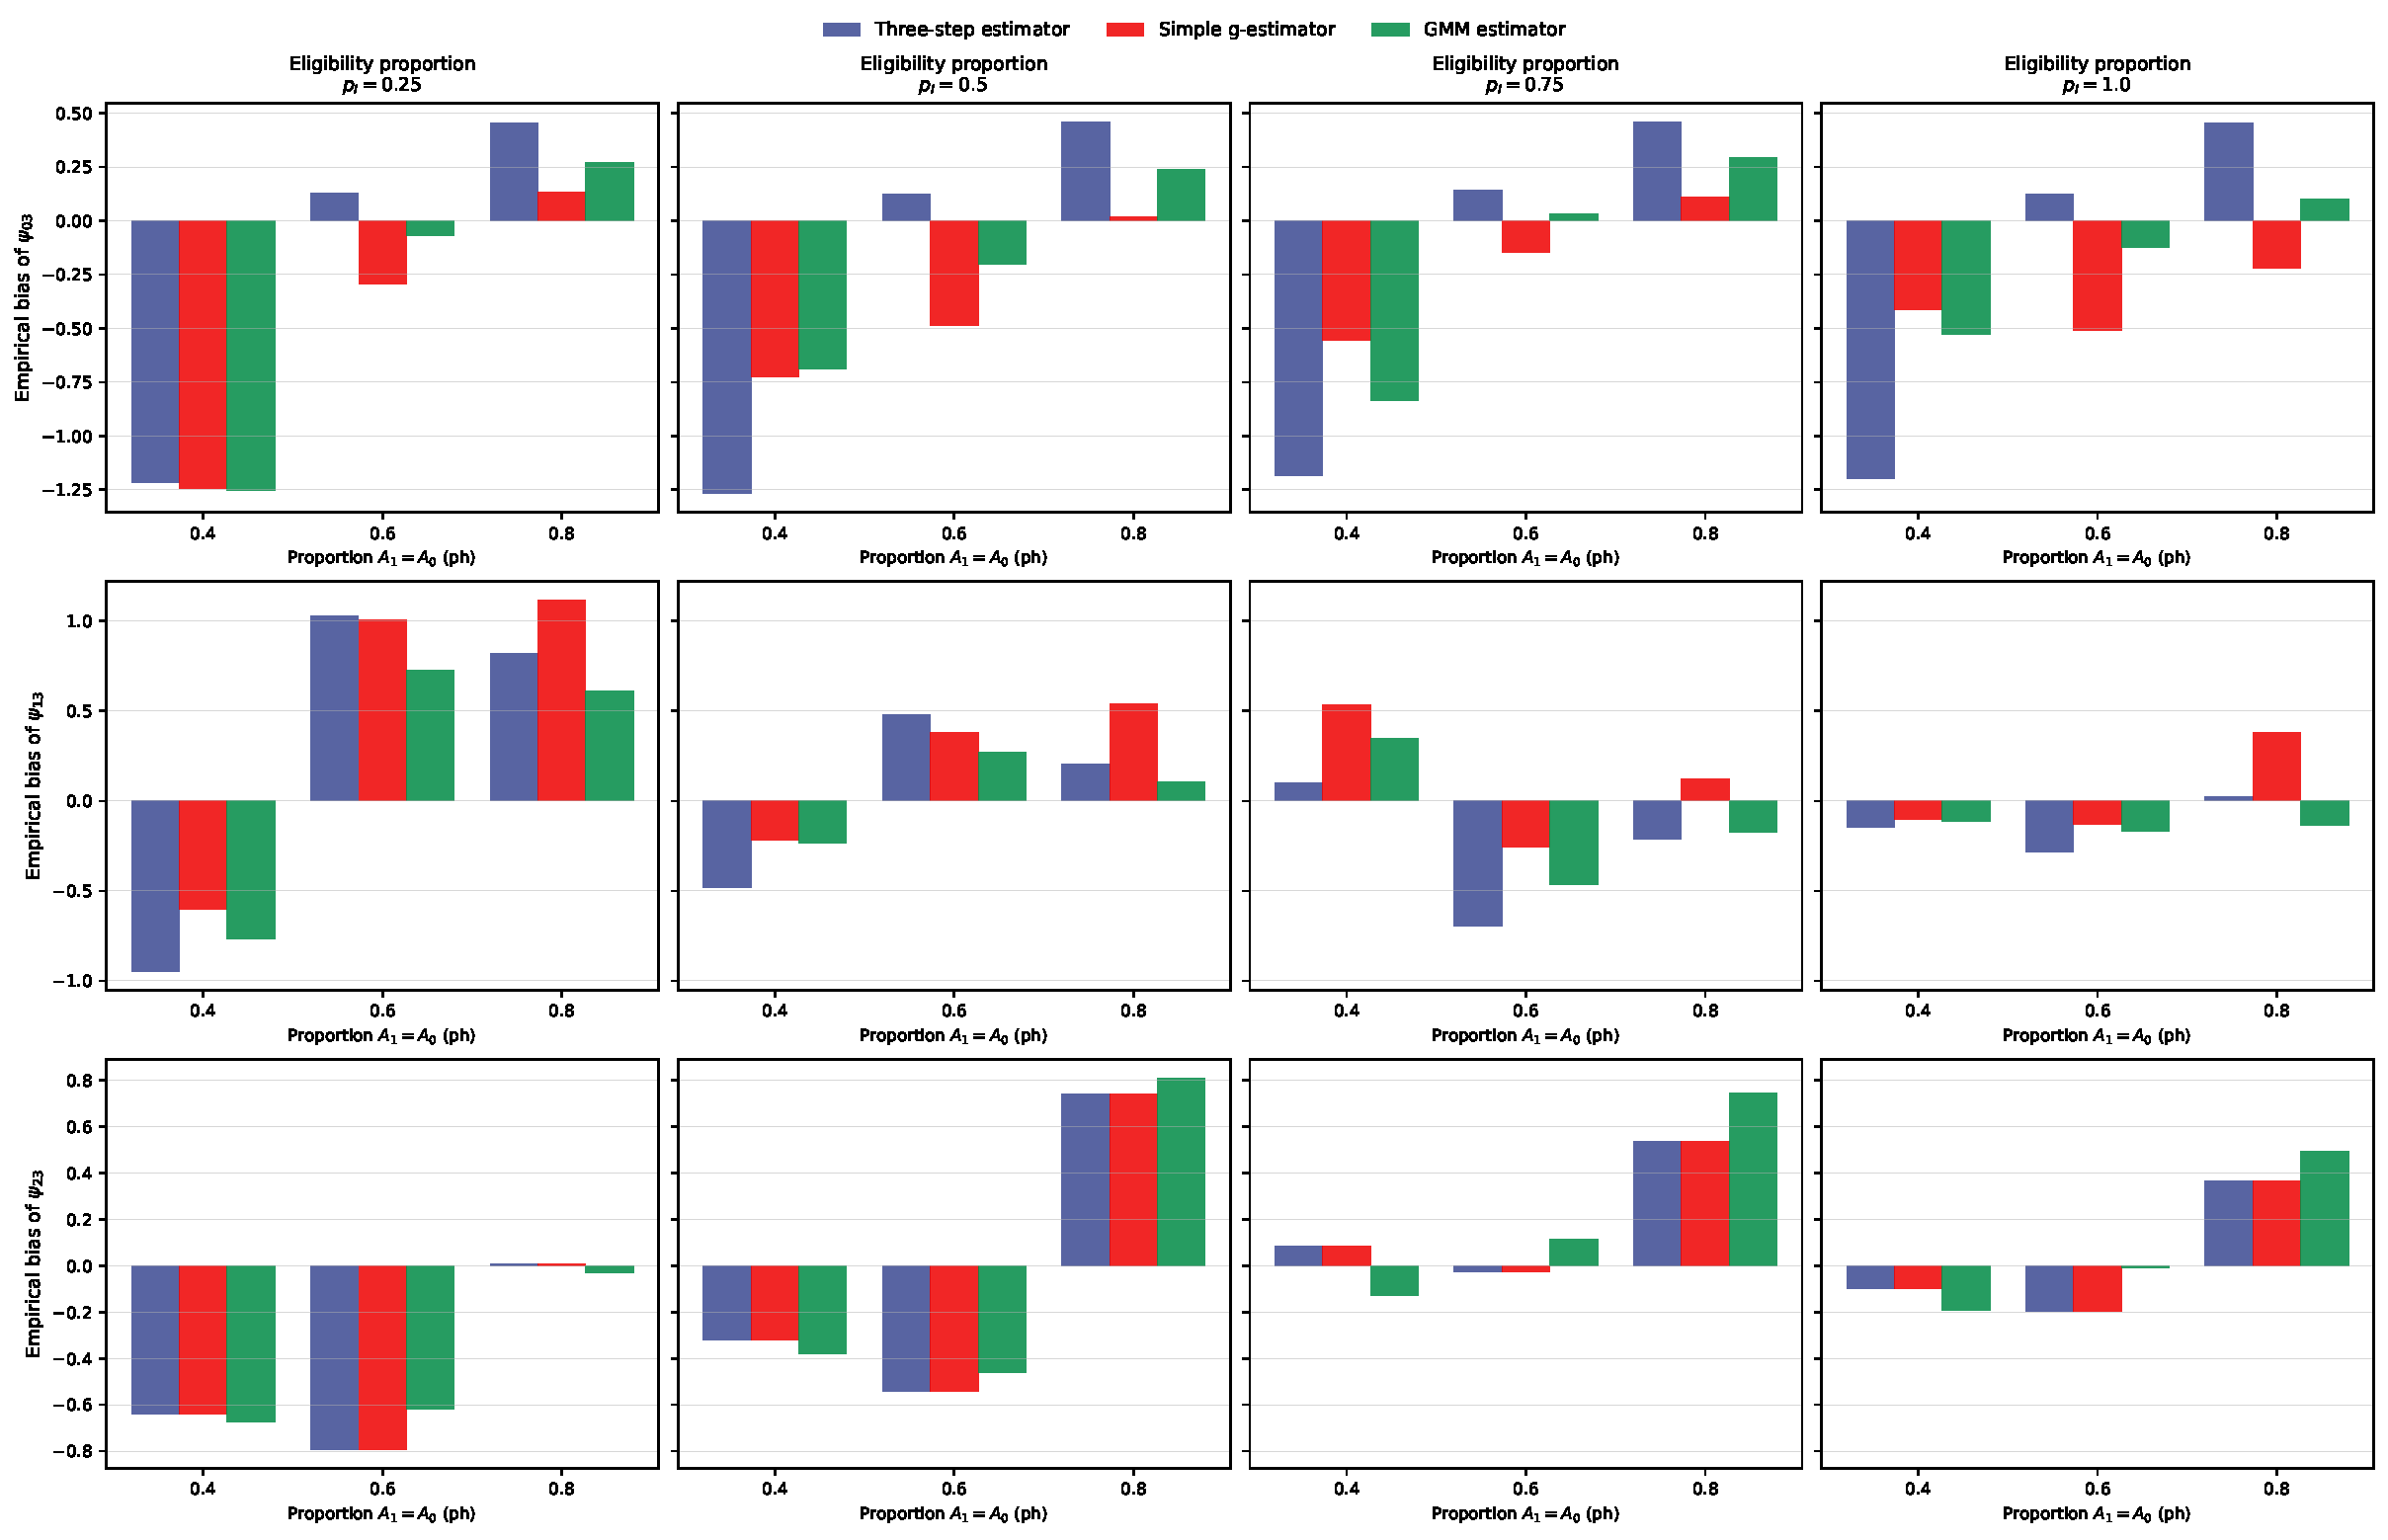
\includegraphics[width=\textwidth]{three_time_continuous/psi1_python_sigma20/simulation_results_plots_bias.pdf}
  \caption{S5 (continuous DGP, $\sigma=20$, $\psi=1$) --- Empirical bias of
           $\hat\psi_{03}$, $\hat\psi_{13}$, and $\hat\psi_{23}$ (rows) as a function
           of $p_h$, stratified by $p_I$ (columns).  Biases are substantially larger
           than in S4 ($\sigma=10$), scaling approximately proportionally with $\sigma$.}
  \label{fig:s5_bias}
\end{figure}

\begin{figure}[htbp]
  \centering
  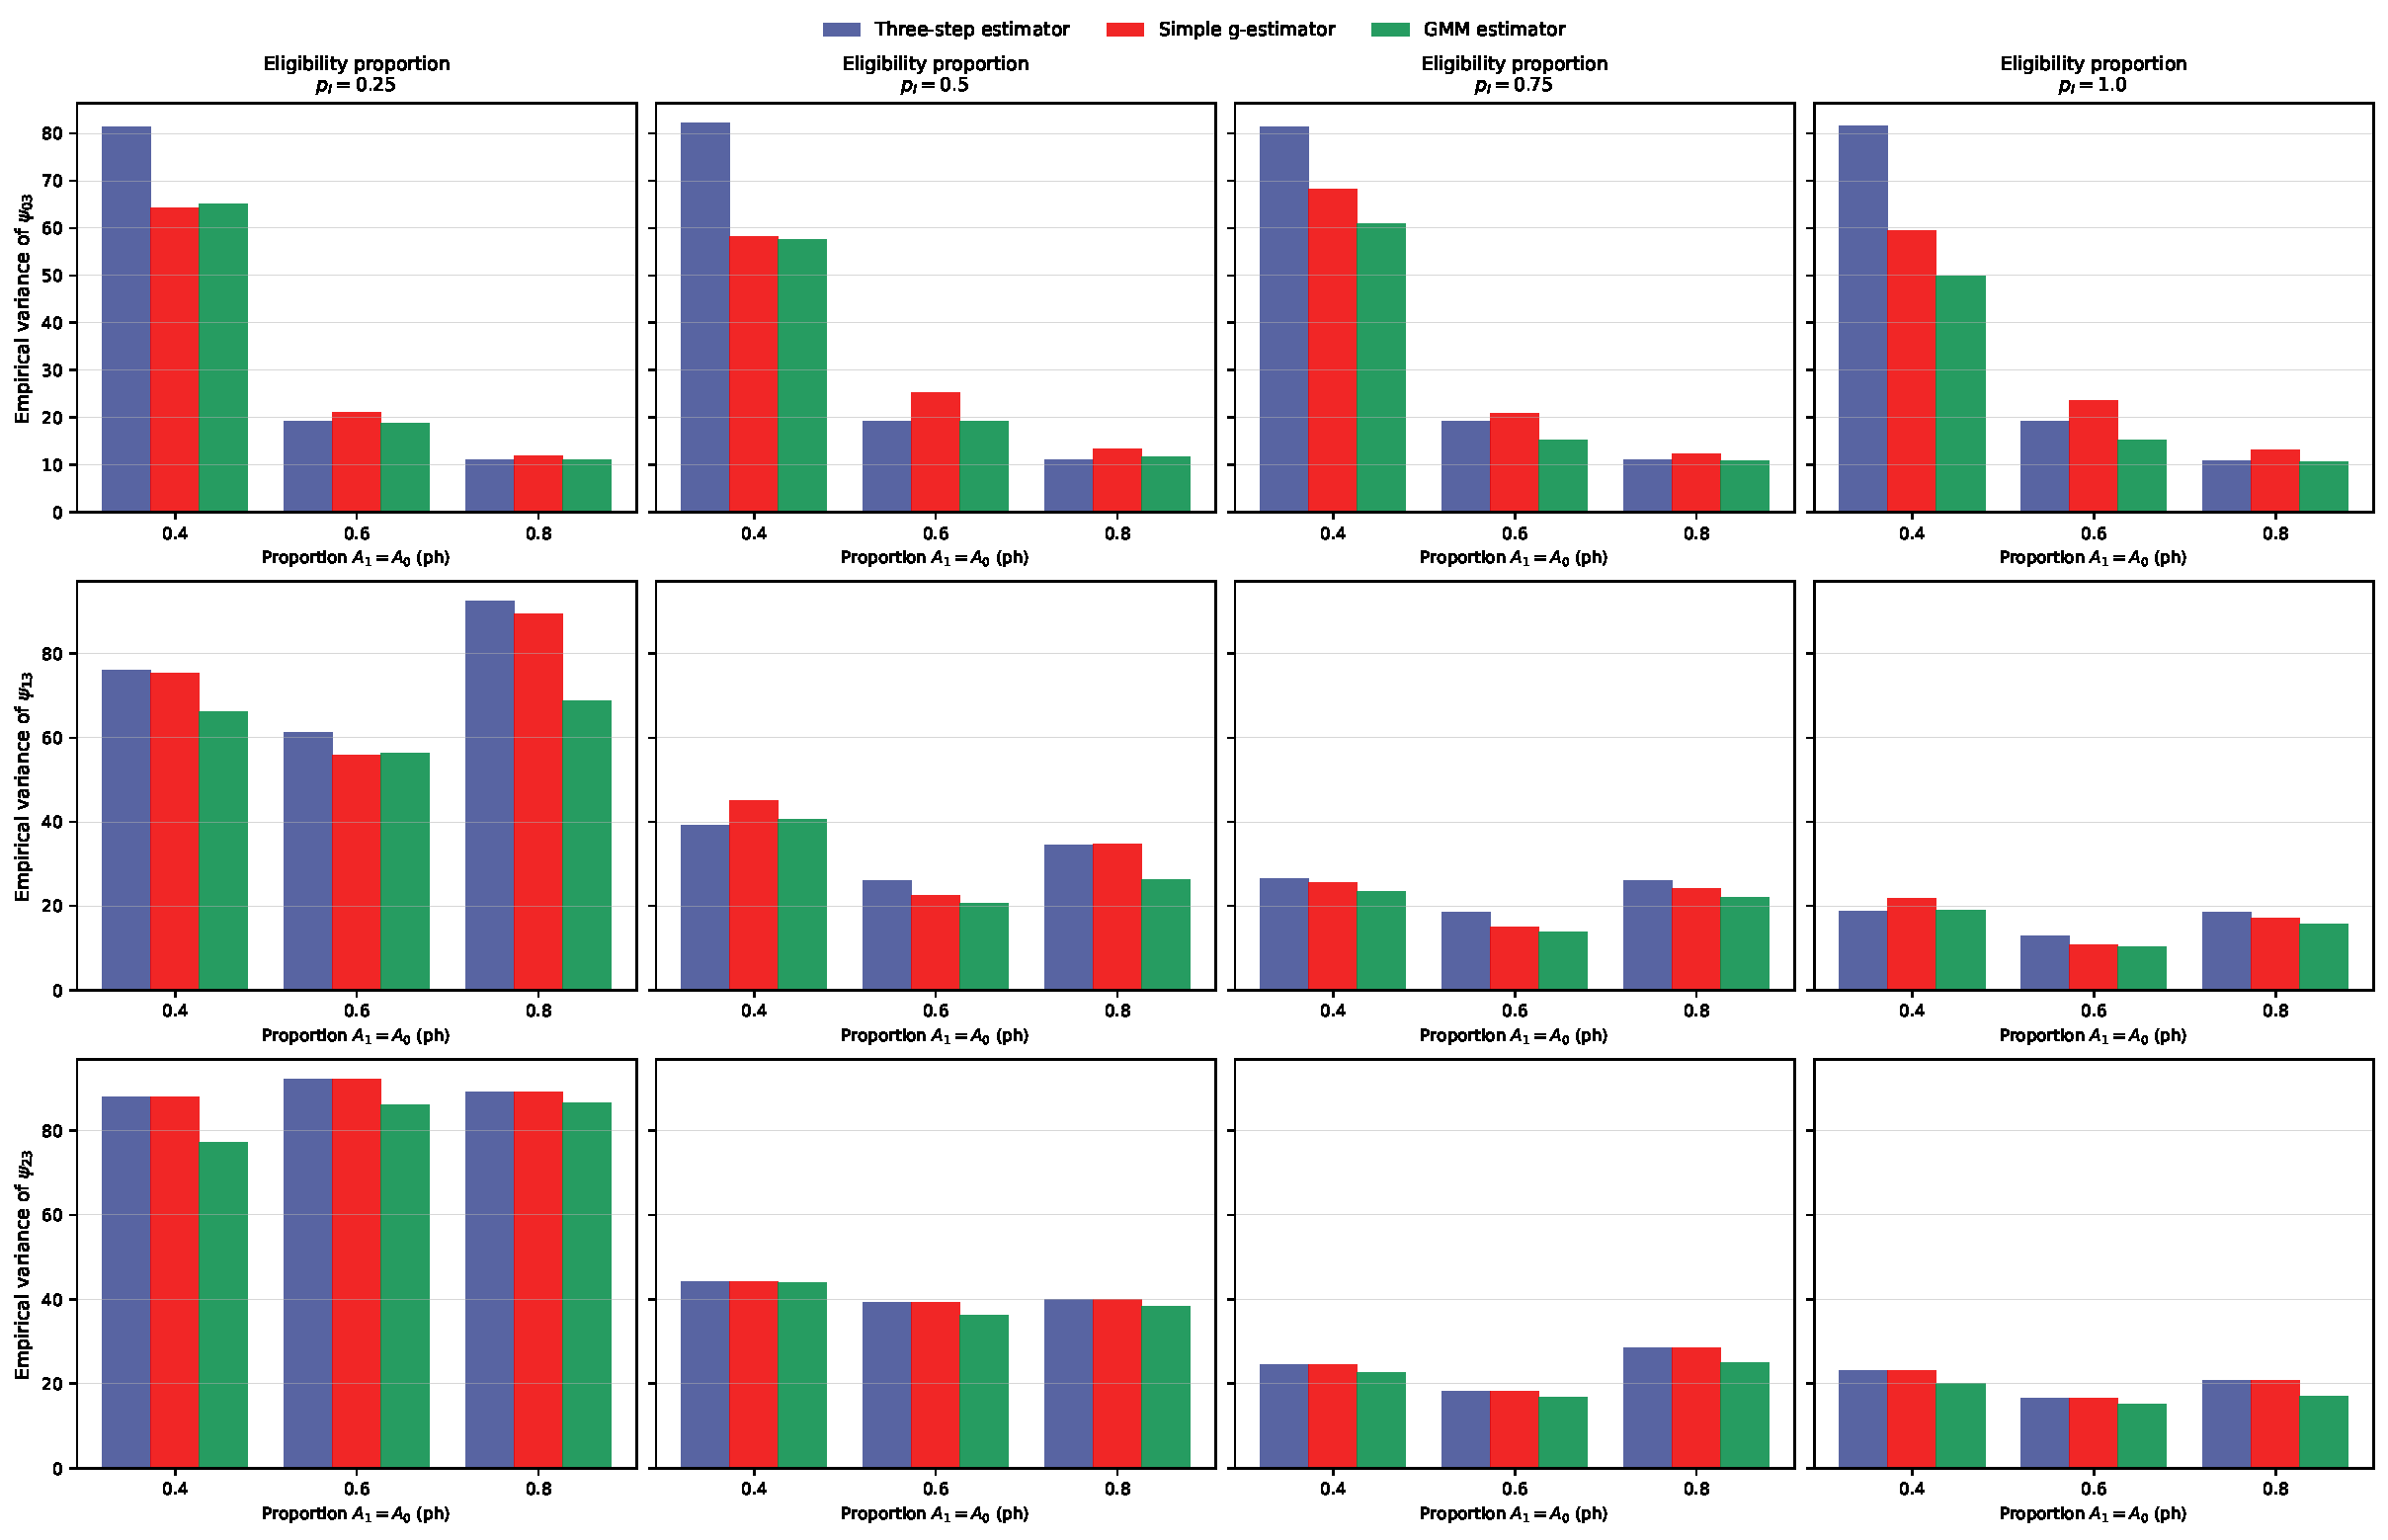
\includegraphics[width=\textwidth]{three_time_continuous/psi1_python_sigma20/simulation_results_plots_variance.pdf}
  \caption{S5 (continuous DGP, $\sigma=20$, $\psi=1$) --- Empirical variance of
           $\hat\psi_{03}$, $\hat\psi_{13}$, and $\hat\psi_{23}$ (rows) as a function
           of $p_h$, stratified by $p_I$ (columns).  Variances are roughly four times
           larger than in S4, consistent with $O(\sigma^2)$ variance scaling.}
  \label{fig:s5_var}
\end{figure}

%%==========================================================================
\section{Summary of Key Findings}
%%==========================================================================

\paragraph{Effect of eligibility proportion ($p_I$).}
Across all scenarios, increasing $p_I$ (more eligible subjects) reduces
both bias and Monte Carlo variance for $\hat\psi_{13}$ and $\hat\psi_{23}$,
since these parameters are identified exclusively from eligible individuals
($I_t=1$).  The estimating equations for $\psi_{03}$ involve all subjects,
so they are less sensitive to $p_I$.

\paragraph{Effect of treatment-hold probability ($p_h$).}
The relationship between $p_h$ and variance is non-monotone.  At
$p_h=0.4$ (frequent switching), variance of $\hat\psi_{03}$ is large
because treatment history is diverse but the baseline covariate $L_0$
is only weakly predictive under high switching.  At $p_h=0.8$
(high persistence), the treatment contrast $A_t - A_{t-1}$ is near
zero for most subjects, reducing identification of the blip parameters
and inflating variance of $\hat\psi_{13}$ and $\hat\psi_{23}$.
Intermediate $p_h=0.6$ generally yields the best variance profile.


\end{document}
